

%%%%%%%%%%%%%%%%%%%%%%%%%%%%%%%%%%%%%%%%%%%%%%%%%%%%%%%%%%%%%%%%%%%%%%%%
%    INSTITUTE OF PHYSICS PUBLISHING                                   %
%                                                                      %
%   `Preparing an article for publication in an Institute of Physics   %
%    Publishing journal using LaTeX'                                   %
%                                                                      %
%    LaTeX source code `ioplau2e.tex' used to generate `author         %
%    guidelines', the documentation explaining and demonstrating use   %
%    of the Institute of Physics Publishing LaTeX preprint files       %
%    `iopart.cls, iopart12.clo and iopart10.clo'.                      %
%                                                                      %
%    `ioplau2e.tex' itself uses LaTeX with `iopart.cls'                %
%                                                                      %
%%%%%%%%%%%%%%%%%%%%%%%%%%%%%%%%%%
%
%
% First we have a character check
%
% ! exclamation mark    " double quote  
% # hash                ` opening quote (grave)
% & ampersand           ' closing quote (acute)
% $ dollar              % percent       
% ( open parenthesis    ) close paren.  
% - hyphen              = equals sign
% | vertical bar        ~ tilde         
% @ at sign             _ underscore
% { open curly brace    } close curly   
% [ open square         ] close square bracket
% + plus sign           ; semi-colon    
% * asterisk            : colon
% < open angle bracket  > close angle   
% , comma               . full stop
% ? question mark       / forward slash 
% \ backslash           ^ circumflex
%
% ABCDEFGHIJKLMNOPQRSTUVWXYZ 
% abcdefghijklmnopqrstuvwxyz 
% 1234567890
%
%%%%%%%%%%%%%%%%%%%%%%%%%%%%%%%%%%%%%%%%%%%%%%%%%%%%%%%%%%%%%%%%%%%
%
\documentclass[twocolumn,11pt,a4paper]{article}		%<-use this for checking equation length
% \documentclass[12pt]{iopart} 

%<-comment out this for checking equations (author list too)
% \usepackage{iopams,setstack} 
%<-comment out this for checking equations
\usepackage{graphicx}
\usepackage{algorithm, algorithmicx, algpseudocode} 
\usepackage{color} 
%This is to decrease the space in subfigure command
\usepackage[tight,scriptsize]{subfigure}
\makeatletter
\renewcommand{\subfigtopskip}{1\p@}
\renewcommand{\subfigcapskip}{0\p@}
\renewcommand{\subfigcaptopadj}{1\p@}
\renewcommand{\subfigbottomskip}{1\p@}
\renewcommand{\subfiglabelskip}{0.05em plus 0.02em minus 0.01em}
\makeatother
% \usepackage{pstool}
\renewcommand{\subcapsize}{\small}
 \usepackage{anysize}							%<-use this for checking equation length
 % \marginsize {1.7cm}{1.5cm}{0.3cm}{0.8cm}			%<-use this for checking equation length
 %  \setlength{\columnsep}{0.5cm}					%<-use this for checking equation length
  \usepackage{amsmath}
\usepackage{amssymb,amsfonts} 			%<-use this for checking equation length
\newcommand{\parham}[1]{\textsf{\emph{\textbf{\textcolor{blue}{#1}}}}} 
\newcommand{\mike}[1]{\textsf{\emph{\textbf{\textcolor{red}{#1}}}}} 
\newcommand{\dean}[1]{\textsf{\emph{\textbf{\textcolor{green}{#1}}}}}
\newcommand{\ken}[1]{\textsf{\emph{\textbf{\textcolor{magenta}{#1}}}}}
\begin{document}

% \begin{document}

\title[State and Parameter Estimation for Spatio-Temporal Neural Fields]{State and Parameter Estimation for Spatio-Temporal Neural Fields}

\author{Dean R. Freestone$^{1,5}$, Parham Aram$^2$, Michael Dewar$^3$, Kenneth Scerri$^4$, David B. Grayden$^{1,5}$, and Visakan Kadirkamanathan$^2$}

% \address{$^1$ Department of Electrical and Electronic Engineering, University of Melbourne, Melbourne, VIC 3010 Australia} \address{$^2$ Department of Automatic Control and Systems Engineering, University of Sheffield, Mappin Street, Sheffield, S1 3JD, UK} \address{$^3$ Department of Applied Physics and Applied Mathematics, Columbia University, NY, USA} \address{$^4$ Department of Systems and Control Engineering, University of Malta, Msida, MSD 1333, Malta} \address{$^5$ The Bionic Ear Institute, East Melbourne, VIC 3002
%  Australia} \ead{dfreestone@bionicear.org} 

\begin{abstract}
	This paper presents a framework for creating patient-specific neural field models from electrophysiological data. The Wilson and Cowen or Amari style neural field equations are used to form a parametric model, where the parameters are estimated from data. To illustrate the estimation framework, data is generated using the neural field equations incorporating modelled sensors, so a comparison can be made between estimated and true parameters. To facilitate state and parameter estimation, we introduce a method to reduce the continuum neural field model, using a basis function decomposition, to form a finite dimensional state-space model. Spatial frequency analysis methods are introduced for model selection, by systematically specifying the basis function configuration required to capture the dominant characteristics of the neural field. We use the reduced model to estimate the state and parameters of the non-reduced model. The estimation procedure consists of a two-stage algorithm incorporating the unscented Rauch Tung Striebel Smoother for state estimation, and a least squares algorithm for parameter estimation. The results show that it is possible to reconstruct the neural field and estimate intracortical connectivity and synaptic time constant with the proposed framework. The results also illustrate the cost of the model reduction with a loss of the high spatial frequency information. This framework provides a link between patient-specific neurophysiological data and theoretical neural fields models. This link may lead to greater understanding of cortical dynamics at the meso/macroscopic scale where diseases such as epilepsy are manifested.   
\end{abstract}

%Uncomment for PACS numbers title message
%\pacs{00.00, 20.00, 42.10}
% Keywords required only for MST, PB, PMB, PM, JOA, JOB? 
%\vspace{2pc}
%\noindent{\it Keywords}: Article preparation, IOP journals
% Uncomment for Submitted to journal title message
%\submitto{\JPA}
% Comment out if separate title page not required
\maketitle

\section{Introduction} This paper presents a theoretical framework for generating patient-specific macroscopic neural field mathematical models from data. There has been much interest in generating physiologically plausible neural field models to study brain dynamics at the meso/macroscopic scale. While our understanding of the function of neurons is well developed, the overall behaviour of the brain's meso and macro-scale dynamics remains largely theoretical. Understanding the brain at this level is extremely important since it is this scale at which pathologies such as epilepsy, Parkinson's disease and schizophrenia are manifested. Mathematical neural field models provide insights into the underlying physics and dynamics of electroencephalography (EEG) and magnetoencephalography (MEG) (see \cite{Deco2008,David2003} for recent reviews). These models have demonstrated possible mechanisms for the genesis of neural rhythms (such as the alpha and gamma rhythms) \cite{Liley1999,RENNIE2000}, epileptic seizure generation \cite{DaSilva2003,Suffczynski2004,Wendling2005} and insights into other pathologies \cite{Moran2008,Schiff2009} that would be difficult to gain from experimental data alone. 

Unfortunately, the use of these models in the clinic has been limited, since they are constructed for ``general'' brain dynamics whereas pathologies almost always have unique underlying patient specific causes. Patient specific data from EEG is readily available in the clinical setting, suggesting an opportunity to make the patient-specific link to models of cortical dynamics. However the meso/macroscopic neural dynamic state is not directly observable in EEG data, making predictions of the underlying physiology inherently difficult.

For models to be clinically viable they must be patient-specific. A possible approach to achieve this would be to fit a general continuum neural field model, like the Wilson and Cohen (WC)~\cite{Wilson1973} or Amari~\cite{Amari1977} models or a neural mass model like the Jansen and Ritt model~\cite{Jansen1995} to patient-specific EEG data. Fitting the neural models to individuals is a highly non-trivial task and until very recently, has not been reported in the literature. 

An estimation framework for neural field models known as dynamical causal modelling (DCM) \cite{David2003,David2006} has recently been proposed for studying evoked potential dynamics. Via a Bayesian inference scheme, DCM estimates the long range connectivity structure between the specific isolated brain regions that best explains a given data set under the Jansen and Ritt equations. Another recent publication describing a parameter estimation method with a neural field model used an unscented Kalman filter with the WC neural field equations \cite{schiff2008kalman}. This work takes a system theoretic approach to the neural estimation problem, successfully demonstrating that it is possible to perform state estimation of modified WC equations. This marks the first step in what has the potential to revolutionise the treatment of many neurological diseases where therapeutic electrical stimulation is viable.

%Currently available epileptic seizure control devices (i.e., the vagal nerve stimulator) are implemented in an ``open loop". That is, the therapeutic electrical stimulation waveforms are adjusted for each patient by trial and error, disregarding the patient's neuro-dynamics and information about their particular pathologies. Given access to an accurate model, the application of optimal control theory in these circumstances would allow for robust therapeutic stimulations.

This paper extends the work of Schiff and Sauer~\cite{schiff2008kalman} by establishing a framework for estimating the state of the WC equations for larger scale (more space) systems via a systematic model reduction procedure. In addition, a method is presented for estimating the connectivity structure and the synaptic time constant. Until now, estimation of local intracortical connectivity structure has not been reported (to the best of the authors knowledge). Recently, it has been shown that it is possible to estimate local coupling of spatiotemporal systems using techniques from control systems theory and machine learning \cite{Dewar2009}. The key development from this recent paper was to represent the spatiotemporal system as a standard state-space model, with the number of states independent of the number of observation locations (recording electrodes in this case). In addition, the appropriate model selection tools have been developed \cite{Scerri2009} allowing for the application of the technique to neural fields. 

Modelling the neural dynamics within this framework has a distinct advantage over the more standard multivariate auto-regressive (AR) models: that the number of parameters to define the spatial connectivity is considerably smaller than the number of AR coefficients typically required to achieve the required model complexity. 

In this paper, we demonstrate for the first time how intracortical connectivity can be inferred from data, based on a variant of the Wilson and Cowan neural field model \cite{Wilson1973}. This work provides a fundamental link between the theoretical advances in neural field modelling and patient-specific data.

The paper proceeds by first deriving the continuum neural field equations in Section~\ref{NeuralModelSection}. Next, a reduced finite dimensional neural field model is derived. The model is reduced by approximating the neural field using a set of continuous basis functions, weighted by a finite dimensional state vector. Section~\ref{SpectralAnalysisSection} establishes conditions using spatial frequency analysis for both sensor and basis function spacing and width, such that the dominant dynamics of the neural field can be represented by the reduced model. The state and parameter estimation procedure is described in Section~\ref{StateAndParameterEstimationSection}. The results for the spatial frequency analysis and parameter estimation are then presented in Section~\ref{ResultsSection}. The implications and limitations of this framework are discussed in Section~\ref{DiscussionSection} along with planned future developments.

\section{Neural Field Model}\label{NeuralModelSection} In this section, we describe a variant of the WC neural field model that was used to create our intracortical connectivity estimator. Neural field models relate mean firing rates of pre-synaptic neural populations to mean post-synaptic membrane potentials. They are popular due to being parsimonious yet having a strong link with the underlying physiology. Each neural population represents a functional cortical processing unit, such as a column. The columnar organisation of the cortex is continuous, where pyramidal cells are members of many columns. In general, cortical structure can be modelled in a physiologically plausible manner as being locally homogeneous (in short range intracortical connectivity) and heterogeneous (in long range cortico-cortical and corticothalamic connectivity)~\cite{Jirsa2009,Qubbaj2007}. In certain regions of the cortex, each column is thought to be connected locally via symmetric short range local excitation, with surround inhibition \cite{Braitenberg1998}. For example, this structural organisation is most studied in the visual system, where the surrounding inhibition effectively tunes a cortical column to a particular receptive visual field~\cite{Sullivan2006}. Neural field models are descriptive of a range of neurodynamics of the cortex such as evoked potentials, visual hallucinations, and epileptic behaviour~\cite{David2003,Bressloff2001,Breakspear2006}. Field models are also capable of generating complex patterns of activity such as Turing patterns, spirals, and travelling oscillations~\cite{Amari1977,Coombes2005,Coombes2007}.

\subsection{Derivation of the Integro-Difference Equation Representation}
The model relates the average number of action potentials $g(\mathbf{r},t)$ arriving at position $\mathbf{r}$ to the local post synaptic membrane voltage $v(\mathbf{r},t)$. The post-synaptic potentials generated at a neuronal population at location $\mathbf{r}$ by action potentials arriving from all other connected populations at locations $\mathbf{r}'$ can be described by 
\begin{equation}
	\label{SpikesToPotential} v\left( {\mathbf{r},t} \right) = \int_{ - \infty }^t {h\left( {t - t'} \right)g\left( {\mathbf{r},t'} \right)dt'}. 
\end{equation}
The post-synaptic response kernel $h(t)$ is described by 
\begin{equation}
	\label{SynapticRespKernel} h(t) = \eta(t)\exp{\left(-\zeta t\right)}. 
\end{equation}
where $\zeta=\tau^{-1}$ and $\tau$ is the synaptic time constant and $\eta(t)$ is the Heaviside step function. Nonlocal interactions between cortical populations are described by 
\begin{equation}
	\label{RateBasedInteractions} g\left( \mathbf{r},t \right) = \int_\Omega {w\left( \mathbf{r},\mathbf{r}' \right)f\left( v\left( \mathbf{r}',t \right) \right)d\mathbf{r}'}, 
\end{equation}
where $f(\cdot)$ is the firing rate function, $w(\cdot)$ is the spatial connectivity kernel, and $\Omega$ is the spatial domain, representing a cortical sheet or surface. The connectivity kernel is typically a ``Mexican hat'' function which describes strong local activation, weak mid-range repression and weak long-range activation. The exact shape of this kernel is assumed to vary across patients, and hence needs to be inferred from data. \ken{Risky comment if we don't get better estimates.}
\begin{figure}[ th]\label{fig:2d_kernel}
   	\begin{center}
   		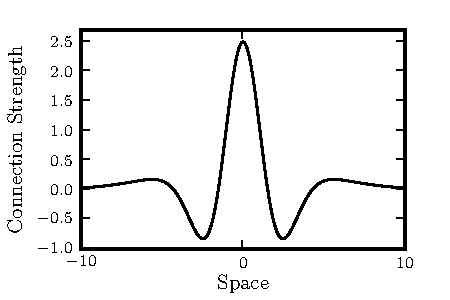
\includegraphics{./Graph/Cross_section_kernel.pdf} 
   	\end{center}
   	\caption{Kernel centred at zero as a function of space.} 
   \end{figure}
The firing rate of the presynaptic neurons is related to the postsynaptic membrane potential by the sigmoidal activation function 
\begin{equation}
	\label{ActivationFunction} f\left( v\left( \mathbf{r}', t \right) \right) = \frac{f_{max}}{1 + \exp \left( \varsigma \left( v_0 - v\left(\mathbf{r}',t\right) \right) \right)}. 
\end{equation}
The parameters $f_{max}$ and $v_0$ describe the maximum firing rate and firing threshold of the neural populations. The parameter $\varsigma$ governs the slope of the sigmoid. By substituting equation~\ref{RateBasedInteractions} into \ref{SpikesToPotential} we get the spatiotemporal model 
\begin{eqnarray}
	\label{FullDoubleIntModel} v\left(\mathbf{r},t\right) &=&  \int_{-\infty}^t h\left(t - t'\right) \\
	&\times&\int_\Omega w\left(\mathbf{r},\mathbf{r}'\right) f\left( v\left( \mathbf{r}',t \right)\right)d\mathbf{r}'dt'. \nonumber
\end{eqnarray}
To arrive at the final form of the model we shall express the synaptic response kernel as a Green's function 
\begin{equation}
	\label{GreensFuncDef} Dh\left( t \right) = \delta \left( t \right), 
\end{equation}
where $D=\frac{d}{dt} + \zeta$ is a temporal differential operator and $\delta(t)$ is the Dirac-delta function giving 
\begin{eqnarray}
	\label{FinalFormContinuous} \frac{dv\left( \mathbf{r},t \right)}{dt} &+& \zeta v\left( \mathbf{r},t \right) = \\
	&&\int_\Omega {w\left( \mathbf{r},\mathbf{r}' \right)f\left( {v\left( \mathbf{r}',t \right)} \right)d\mathbf{r}'}. \nonumber
\end{eqnarray}
To arrive at the integro-difference equation (IDE) form of the model we discretise time using a first-order Euler method (see~\ref{Time Discretization}) giving 
\begin{eqnarray}
	\label{DiscreteTimeModel} v_{t+T_s}\left(\mathbf{r}\right) &=& \xi v_t\left(\mathbf{r}\right) + T_s \int_\Omega { w\left(\mathbf{r},\mathbf{r}'\right) f\left(v_t\left(\mathbf{r}'\right)\right) d\mathbf{r}'} \nonumber\\ 
	&+& e_t\left(\mathbf{r}\right), 
\end{eqnarray}
where $T_s$ is the time step, $\xi = 1-\zeta T_s$ and $e_t(\mathbf{r})$ is an i.i.d. disturbance such that $e_t\sim\mathcal{GP}(\mathbf 0,\gamma(\mathbf{r}-\mathbf{r}'))$. Here $\mathcal{GP}(\mathbf 0,\gamma(\mathbf{r}-\mathbf{r}'))$ denotes a spatial Gaussian Process with mean zero and covariance function $\gamma(\mathbf{r}-\mathbf{r}')$~\cite{Rasmussen2005}. This term is added to account for uncertainty in the model. To simplify the notation, the index of the future time sample, $t+T_s$, shall be referred to as $t+1$ throughout the rest of the paper. The mapping between the membrane voltage and the collected iEEG/LFP data is modelled using the observation function 
\begin{equation}
	\mathbf{y}_t = \int_{\Omega}{m\left(\mathbf{r}_n-\mathbf{r}'\right)v_t\left(\mathbf{r}'\right)d\mathbf{r}'} + \boldsymbol{\varepsilon}_t, 
\end{equation}
where $\mathbf{r}_n$ defines the location of the sensors in the field, $n=1,...,N$ indexes the sensors, $\boldsymbol{\varepsilon}_t \sim \mathcal{N}\left(0,\Sigma_{\varepsilon}\right)$ and $\mathcal{N}\left(0,\Sigma_{\varepsilon}\right)$ denotes the multivariate Normal distribution with mean zero and covariance matrix $\Sigma_{\varepsilon}$. The output kernel $m(\mathbf{r}-\mathbf{r}')$ governs the sensor pick-up geometry where 
\begin{equation}
	m\left(\mathbf{r}-\mathbf{r}'\right) = \exp{\left(-\frac{(\mathbf{r}-\mathbf{r}')^\top(\mathbf{r}-\mathbf{r}')}{\sigma_m^2}\right)}. 
\end{equation}

\subsection{Derivation of Finite Dimensional State-Space Model} 
In order to implement standard estimation techniques, we use a decomposition of the field using a set of Gaussian basis functions that are defined by
\begin{equation}\label{eq:FieldBasisFunction}
	\phi\left(\mathbf{r}-\mathbf{r}'\right) =
\exp{\left(-\frac{(\mathbf{r}-\mathbf{r}')^\top(\mathbf{r}-\mathbf{r}')}{\sigma_{\phi}^2}\right)}. 
\end{equation}
Decomposition allows a continuous field to be represented by a finite dimensional state vector. This facilitates application of standard nonlinear state estimation methods such as the unscented Kalman filter. The field decomposition is described by 
\begin{equation}
	\label{DefFieldDecomp} v_t\left(\mathbf{r}\right) \approx \boldsymbol{\phi}^{\top}\left(\mathbf{r}\right) \mathbf{x}_t, 
\end{equation}
where $\mathbf{\boldsymbol{\phi}}(\mathbf{r})$ is a vector of Gaussian basis functions that are scaled by the state vector, $\mathbf{x}_t$. The choice of Gaussian basis functions can be justified by the existence of the so called bump solutions for this class of model, which have a Gaussian shape~\cite{Coombes2005}. The width and positioning of the basis functions can be determined by spectral analysis (explained in detail in Section~\ref{SpectralAnalysisSection}). The connectivity kernel can also be decomposed as 
\begin{equation}\label{DefKernelDecomp}
	 w\left(\mathbf{r},\mathbf{r}'\right) =\boldsymbol{\psi}^\top\left(\mathbf{r},\mathbf{r}'\right) \boldsymbol{\theta},
\end{equation}
where $\boldsymbol{\psi}(r,r')$ is a vector of Gaussian basis functions and $\boldsymbol{\theta}$ is a vector of scaling parameters. By assuming a Gaussian isotropic connectivity structure the kernel basis functions can be written as $\psi(\mathbf{r}-\mathbf{r}')$. We will assume that we know the parametric form of the connectivity basis functions, where the scaling parameters $\boldsymbol{\theta}$ are unknown. Each connectivity basis function can, individually, be considered a layer in the Wilson and Cowan model, representing short range excitation, surround inhibition and mid-range excitation. Making substitutions of equations~\ref{DefFieldDecomp} and~\ref{DefKernelDecomp} into~\ref{DiscreteTimeModel} we get 
\begin{eqnarray}
	\label{reduced continuous model}\boldsymbol{\phi}^{\top}(\mathbf{r})\mathbf{x}_{t+1}&=& T_s\int_\Omega{f(\boldsymbol{\phi}^{\top}(\mathbf{r}')\mathbf{x}_t )\boldsymbol{\psi}^{\top}(\mathbf{r}-\mathbf{r}')d\mathbf{r}'}\boldsymbol{\theta}\nonumber \\ 
	&+& \xi\boldsymbol{\phi}^{\top}(\mathbf{r})x_t + e_t(\mathbf{r}). 
\end{eqnarray}
Next we multiply equation~\ref{reduced continuous model} by $\boldsymbol{\phi}(r)$ and integrate over the spatial domain $\Omega$ to get 
\begin{eqnarray}
	\label{StartofReduction}\lefteqn{ \int_\Omega {\boldsymbol{\phi} \left(\mathbf{r}\right)\boldsymbol{\phi}^{\top}\left(\mathbf{r}\right) d\mathbf{r}} \mathbf{x}_{t+1}=} \nonumber\\
 &&T_s \int_\Omega {\boldsymbol{\phi} (\mathbf{r}) \boldsymbol{\theta}^{\top} \int_\Omega {\boldsymbol{\psi} \left(\mathbf{r}-\mathbf{r}'\right) f\left(\boldsymbol{\phi}^{\top}\left(\mathbf{r}'\right) \mathbf{x}_t \right)d\mathbf{r}'}d\mathbf{r}} \nonumber\\
&+& \xi\int_\Omega {\boldsymbol{\phi}(\mathbf{r})\boldsymbol{\phi}^{\top}(\mathbf{r})d\mathbf{r}} \mathbf{x}_t+
\int_\Omega{\boldsymbol{\phi} \left(\mathbf{r}\right) e_t\left(\mathbf{r}\right)d\mathbf{r}}. 
\end{eqnarray}
Now defining
\begin{equation}\label{eq:DefGamma}
	\boldsymbol{\Gamma} = \int_\Omega {\boldsymbol{\phi} \left(\mathbf{r}\right)\boldsymbol{\phi} ^{\top}\left(\mathbf{r}\right)d\mathbf{r}}, 
\end{equation}
and substituting this into equation~\ref{StartofReduction} and cross-multiplying by $\boldsymbol{\Gamma}^{-1}$ gives 
\begin{eqnarray}\label{eq:ReducedForm}
	 \lefteqn{\mathbf{x}_{t+1} \nonumber = T_s\boldsymbol{\Gamma}^{ - 1}\int_\Omega {\boldsymbol{\phi}(\mathbf{r}) \int_\Omega {f(\boldsymbol{\phi}^{\top}(\mathbf{r}')\mathbf{x}_t) \boldsymbol{\psi}^{\top} (\mathbf{r}-\mathbf{r}')d\mathbf{r}'} d\mathbf{r}} \boldsymbol{\theta}} \nonumber\\
&+&\xi\mathbf{x}_t + \boldsymbol{\Gamma}^{-1} \int_\Omega{\boldsymbol{\phi}(\mathbf{r})e_t(\mathbf{r})d\mathbf{r}}.
\end{eqnarray}
This can be simplified by exploiting the symmetry (isotropy) of the connectivity kernel where
\begin{equation}
	\boldsymbol{\psi} (\mathbf{r}-\mathbf{r}') = \boldsymbol{\psi} (\mathbf{r}'-\mathbf{r}).
\end{equation}
To make the simplification we first define
\begin{equation}\label{eq:DefPsi}
	\boldsymbol{\Psi}(\mathbf{r}') = T_s\boldsymbol{\Gamma}^{-1}\int_\Omega {\boldsymbol{\phi}(\mathbf{r})\boldsymbol{\psi}^{\top} (\mathbf{r}'-\mathbf{r})d\mathbf{r}},
\end{equation}
which is constant and can be defined analytically. Now substituting~\ref{eq:DefPsi} into~\ref{eq:ReducedForm} gives
\begin{equation}
	\mathbf{x}_{t+1} = \int_\Omega \boldsymbol{\Psi}(\mathbf{r}') f(\boldsymbol{\phi}^{\top}(\mathbf{r}')\mathbf{x}_t) d\mathbf{r}' \boldsymbol{\theta} + \xi\mathbf{x}_t + \boldsymbol{\Gamma}^{-1} \int_\Omega{\boldsymbol{\phi}(\mathbf{r})e_t(\mathbf{r})d\mathbf{r}}.
\end{equation}
Now we define the state disturbance as
\begin{equation}\label{eq:AppendixWt} 
	\mathbf{e}_t=\boldsymbol{\Gamma}^{-1}\int_\Omega {\boldsymbol{\phi} ( \mathbf{r} )e_t( \mathbf{r} )d\mathbf{r}} 
\end{equation}
which is a zero mean normally distributed white noise process with covariance (see~\ref{ColoredNoise})
\begin{equation}
	\boldsymbol\Sigma_e =\mathbf{\Gamma}^{-1}\int_{\Omega}\int_{\Omega}\boldsymbol{\phi}\left(\mathbf r\right) \gamma\left(\mathbf r- \mathbf r' \right)\boldsymbol{\phi}\left(\mathbf r'\right)^{\top}d\mathbf r' d\mathbf r\mathbf{\Gamma}^{- \top}. 
\end{equation}
Under the assumption the basis function decomposition is accurate, the observation equation of the reduced model is
\begin{equation}\label{ObservationEquation} 
	\mathbf{y}_t = \mathbf{C}\mathbf{x}_t + \boldsymbol{\varepsilon}_t,
\end{equation}
where the observation matrix is 
\begin{equation}
	\mathbf{C} = \left[
	\begin{array}{{ccc}} 
		c_{1,1} & \dots & c_{1,L} \\
		\vdots & \ddots & \vdots \\
		c_{N,1} & \dots & c_{N,L} 
	\end{array}
	\right] 
\end{equation}
where $L$ is the number of basis functions used to decompose the neural field and 
\begin{equation}
	c_{i,j} = \int_{\Omega}m(\mathbf{r}_i - \mathbf{r}')\boldsymbol{\phi}_j(\mathbf{r}')d\mathbf{r}'. 
\end{equation}
Now we have the final form of the state-space model where
\begin{equation}
	\mathbf{x}_{t+1} = Q(\mathbf{x}_t) +\mathbf{e}_t.
\end{equation}
\begin{equation} 
	\mathbf{y}_t = \mathbf{C}\mathbf{x}_t + \boldsymbol{\varepsilon}_t,
\end{equation}
where 
\begin{equation}\label{eq:QmatrixForSigmapoints}
	Q(\mathbf{x}_t) = \int_\Omega \boldsymbol{\Psi}(\mathbf{r}') f(\boldsymbol{\phi}^{\top}(\mathbf{r}')\mathbf{x}_t) d\mathbf{r}' \boldsymbol{\theta} + \xi\mathbf{x}_t.
\end{equation}

% \begin{equation}
% \mathbf{C} = \left[\begin{array}{{cccc}}
% \int_{\Omega}m(\mathbf{r}_1 - \mathbf{r}')\boldsymbol{\phi}_1(\mathbf{r}')d\mathbf{r}' & \int_{\Omega} m(\mathbf{r}_1 - \mathbf r')\boldsymbol \phi_2(\mathbf r')d\mathbf r' & \dots
% &\int_{\Omega}m(\mathbf r_1 - \mathbf r')\boldsymbol \phi_n(\mathbf
% r')d\mathbf r' \\
% \int_{\Omega}m(\mathbf r_2 - \mathbf r')\boldsymbol \phi_1(\mathbf
% r')d\mathbf r'&\int_{\Omega}m(\mathbf r_2 - \mathbf r')\boldsymbol
% \phi_2(\mathbf r')d\mathbf r'& \dots &\int_{\Omega}m(\mathbf r_2 -
% \mathbf r')\boldsymbol \phi_n(\mathbf r')d\mathbf r'\\
% \vdots&\vdots&\ddots&\vdots\\
% \int_{\Omega}m(\mathbf r_{n_y} - \mathbf r')\boldsymbol \phi_1(\mathbf
% r')d\mathbf r'&\int_{\Omega}m(\mathbf r_{n_y} - \mathbf r')\boldsymbol
% \phi_2(\mathbf r')d\mathbf r'& \dots &\int_{\Omega}m(\mathbf r_{n_y} -
% \mathbf r')\boldsymbol \phi_n(\mathbf r')d\mathbf r'
% \end{array}\right],
% \end{equation}
% and $m(\mathbf r_n - \mathbf{r}')$ is the observation kernel.
\section{Spectral Analysis and Model Selection}\label{SpectralAnalysisSection} Spectral analysis was used to identify both the number of sensors and the number of basis functions required to reconstruct the neural field from sampled observations \cite{Sanner1992,Scerri2009}. Based on a two-dimensional extension of Shannon's sampling theorem \cite{Peterson1962}, the spatial bandwidth of the observed field can be used to provide a lower bound on both the number of sensors and the number of basis functions required to capture the dominant spectral characteristics of the neural field.

Let the spectral representation of the dynamic field at time $t$ be denoted by $V_t(\boldsymbol{\nu})$. Based on Shannon's sampling theorem, for an accurate representation of this field by spatially discrete observations, $V_t(\boldsymbol{\nu})$ needs to be spatially band-limited. Such a condition ensures that $V_t(\boldsymbol{\nu}) \approx 0 ~ \forall \boldsymbol{\nu} > \boldsymbol{\nu}_c$, where $\boldsymbol{\nu}_c$ is a cutoff frequency (typically taken as -3~dB point) with $\boldsymbol{\nu}_c = [\nu_c ~ \nu_c]^\top$. Given such a band-limited field, the distance between adjacent sensors, $\Delta_y$, needs to satisfy 
\begin{equation}
	\label{eq:MinimumSensorDistance} \Delta_y < \frac{1}{2\rho_y\nu_{c}}, 
\end{equation}
where $\rho_y \in \mathbb{R} \ge 1$ is an oversampling parameter. This condition must be satisfied to avoid spectral aliasing effects in the representation of the hidden dynamic field $v_t(\mathbf{r})$ by the sampled observations, $\mathbf{y}_t$.

In practice, it is difficult to estimate the bandwidth of the cortex using traditional electrophysiological measurements thus allowing the positioning of sensor in accordance to equation~\ref{eq:MinimumSensorDistance}. However, we envisage it may be possible to estimate it using other modalities with higher spatial resolution such as, fMRI, NIRS or other optical imaging techniques~\cite{Issa2000}. Nevertheless, using electrophysiological measurements, spectral aliasing can still be avoided by a proper choice of the spatial sampling distance given the sensors spectral characteristics. Sensors with smooth wide spatial responses result in a spectral low-pass action, thus providing spatial anti-aliasing filtering. Such sensors therefore band-limit the field to a known bandwidth, denoted by $\nu_{co}$. Aliasing can then be avoided by positioning the sensors according to equation~\ref{eq:MinimumSensorDistance}, with $\nu_{co}$ replacing $\nu_c$. 

Although such sensors avoid errors due to aliasing, they attenuate the high frequency variations in the observations. Therefore, any procedure applied to estimate the original field or the underlying connectivity structure from these band-limited observations will underestimate the high frequency component in both the field and the kernel. Such a remark motivates the use of sensors with wider bandwidths. Nevertheless, this choice would require an excessive number of sensors in order to satisfy Shannon's sampling theorem for a reasonable spatial region. Therefore, a compromise needs to be found between the bandwidth of the sensor response, the accuracy of the estimation results and the number of sensors used and thus the computational demands of estimation procedure.

Similar considerations need to be made regarding the representation of the dynamic field, $v_t(\mathbf{r})$, using the basis function decomposition. The minimum distance between adjacent basis functions must also satisfy Shannon's sampling theorem to capture the dominant spectral information of the field. Thus, the minimum distance between basis functions must satisfy 
\begin{equation}\label{eq:BasisFunctionSeparation}
	\Delta_{\phi} < \frac{1}{2\rho_{\phi}\nu_{co}}
\end{equation}
where $\rho_{phi}$ is an over-sampling parameter to determine the basis function separation. For the Gaussian basis functions, $\phi(\mathbf{r})$, being considered, the basis function width parameter, $\sigma_{\phi}^2$, can also be inferred using spectral considerations~\cite{Sanner1992,Scerri2009}. The Fourier transform of an \textit{n}-dimensional Gaussian is another Gaussian given by
\begin{equation}\label{eq:GaussianFT}
\boldsymbol\Phi(\boldsymbol \nu)=\left(\frac{1}{\pi\sigma_{\nu}^2}\right)^{\frac{n}{2}}\mathrm{exp}\left(-\frac{1}{\sigma_{\nu}^2}\boldsymbol\nu^\top \boldsymbol\nu\right),
\end{equation}
where 
\begin{equation}\label{eq:GaussianFTWidth}
	\sigma^2_{\nu} = \frac{1}{\pi^2\sigma_{\phi}^2}. 
\end{equation}
The basis function width, $\sigma^2_{\phi}$, should be chosen to give at least 3~dB attenuation at $\boldsymbol\nu_{co}$ giving
\begin{equation}\label{eq:WidthCutOffRelationship}
 \sigma^2_{\phi}= \frac{1}{\pi^2\sigma_{\nu_{co}}^2},
\end{equation}
where
\begin{equation}\label{eq:WidthFrequencyRelationship}
 \sigma^2_{\nu_{co}}= \frac{2\boldsymbol\nu_{co}^\top \boldsymbol\nu_{co}}{\ln 2}.
\end{equation}
This ensures that the basis functions can represent field with frequency content up to $\boldsymbol\nu_{co}$. Proofs for equations~\ref{eq:GaussianFT} and \ref{eq:WidthFrequencyRelationship} are given in~\ref{ap:FrequencyAnalysis}.

Note that for a spatially homogeneous isotropic fields, the basis functions can be placed on a regular grid. Thus, the knowledge of the distance between basis functions directly implies the total number of basis functions required to represent a known spatial region.

% 
% Due to the high dimensionality of the brain and the current electrode systems, we can not expect to have more sensors than basis functions.
\section{State and Parameter Estimation}\label{StateAndParameterEstimationSection} In this section we describe the procedure for estimating the states, $\mathbf{x}_t$, and the connectivity kernel parameters, $\boldsymbol \theta$, and the synaptic time constant, $\xi$. The estimation process is a two part iterative algorithm, consisting of a state estimation step followed by a parameter estimation step. At each iteration, the sequence of estimated state vectors is used to update the parameter set. The resulting parameters are then used to estimate a new state vector sequence for the next iteration. The procedure stops when the parameters converge. The algorithm is initialised using a bounded random state vector sequence that guarantees the initial estimated parameter set forms a stable kernel.

The unscented Rauch Tung Striebel smoother (URTSS)~\cite{Sarkka2010} is used for the state estimation. The URTSS incorporates an unscented Kalman Filter (UKF)~\cite{Julier1997, Merwe2003} in a forward iteration to estimate posterior states, $\hat{\mathbf x}_t^{f}$, followed by a backward iteration to compute the smoothed state estimates, $\hat{\mathbf x}_t^{b}$. The first and the second order moments of the predicted state are captured by propagating the so-called sigma points through the state equation. The sigma points, $\mathcal X_i$, are calculated using the unscented transform as follows:
\begin{equation}\label{eq:sigmapoints1}
	\mathcal X_{0}=\bar x 
\end{equation}
\begin{equation}
	\mathcal X_{i}=\bar x+(\sqrt{( L + \lambda)\mathbf P_x})_i, \quad i=1, \dots, L 
\end{equation}
\begin{equation}\label{eq:sigmapoints2}
	\mathcal X_{i}=\bar x-(\sqrt{( L + \lambda)\mathbf P_x})_{i- L}, \quad i= L+1, \dots, 2 L 
\end{equation}
where $\bar x$ represents either $\hat{\mathbf x}_t^{f}$ or $\hat{\mathbf x}_t^{b}$, $\mathbf{P}_x$ is the corresponding covariance matrix from the filtering or smoothing, $(\sqrt{( L + \lambda)\mathbf P_x})_i$ is the $i$th column of the weighted matrix square root of $\mathbf P_x$ and $L$ is the dimension of the state space. The total number of sigma points is $2L+1$. The scaling parameter, $\lambda$, is defined as 
\begin{equation}\label{eq:sigmapoints3}
	\lambda=\alpha^2( L+\kappa) - L 
\end{equation}
where the constant $\alpha$ determines the spread of the sigma points, $\beta$ incorporates prior knowledge of the distribution of $\mathbf{x}$ and $\kappa$ is a scaling parameter (see ~\cite{Haykin2001} for more details). 

The sigma vectors are propagated through the system equations and weighted to form the predicted mean and covariance. The weights are calculated by 
\begin{equation}
	\mathbf W_0^{(m)}=\frac{\lambda}{ L+\lambda} 
\end{equation}
\begin{equation}
	\mathbf W_0^{(c)}=\frac{\lambda}{ L+\lambda}+(1-\alpha^2+\beta) 
\end{equation}
\begin{equation}
	\mathbf W_i^{(m)}=\mathbf W_i^{(c)}=\frac{1}{2( L+\lambda)} \quad i=1, \dots, 2L. 
\end{equation}
where the superscripts $m$ and $c$ stand for mean and covariance. Since the observation equation is linear (equation~\ref{ObservationEquation}) the standard Kalman Filter update equations are  used to correct the predicted states. The state estimates from the forward filtering are used to form a new set of sigma points for the smoother, as described above. To compute the smoother gain, the predicted cross-covariance matrix of the states is used with the covariance matrix. A summary of the URTSS procedure is given in Algorithm~\ref{UKFAlgorithm}. It should be noted that  the disturbance, $e_t\left(\mathbf{r}\right)$ and the measurement noise, $\boldsymbol{\varepsilon}_t$, are additive. Therefore, the additive form of the URTS is used, otherwise the state vector should be augmented with the noise terms. The additive disturbance form reduces the dimension and the number of sigma points used in the algorithm.
\begin{algorithm}
	\begin{small}
	\caption{The Unscented RTS Smoother}\label{UKFAlgorithm} 
	\begin{algorithmic}[1] 
		\State Forward initialisation 
		\begin{equation*}
		 \hat{\mathbf x}_0, \mathbf P_0 
		\end{equation*}
		\State Forward iteration: for $t \in \left\lbrace 0,\cdots, T\right\rbrace $,
		calculate the sigma points $\mathcal X_{i,t}^f$ using equations \ref{eq:sigmapoints1}-\ref{eq:sigmapoints3} and propagate through equation~\ref{eq:QmatrixForSigmapoints}
% 		\begin{small}
		\begin{equation*}
			\mathcal X_{i,t+1}^{f-}=Q(\mathcal X_{i,t}^f) 
		\end{equation*}
% 		\end{small}
		calculate the predicted state and the predicted covariance matrix
		\begin{equation*}
			\hat{\mathbf x}_{t+1}^{f-}=\sum_{i=0}^{2L} W_i^{(m)}\mathcal X_{i,t+1}^{f-} 
		\end{equation*}
		\begin{equation*}
			\mathbf P_{t +1}^{f-}=\sum_{i=0}^{2L} W_i^{(c)}(\mathcal X_{i,t+1}^{f-}-\hat{\mathbf x}_{t +1}^{f-})(\mathcal X_{i,t+1}^{f-}-\hat{\mathbf x}_{t +1}^{f-})^\top+\boldsymbol \Sigma_e 
		\end{equation*}
		compute the filter gain, the filtered state and the filtered covariance matrix using the standard Kalman Filter update equations
		\begin{equation*}
			\mathcal K_{t+1}=\mathbf P_{t +1}^{f-}\mathbf C ^\top(\mathbf C \mathbf P_{t +1}^{f-}\mathbf C ^\top+\boldsymbol \Sigma_{\epsilon})^{-1} 
		\end{equation*}
		\begin{equation*}
			\hat{\mathbf x}_{t+1}^{f}=\hat{\mathbf x}_{t+1}^{f-}+\mathcal K_{t+1}(\mathbf y_{t+1}-\mathbf C\hat{\mathbf x}_{t +1}^{f-}) 
		\end{equation*}
		\begin{equation*}
			\mathbf P_{t+1}^f=(\mathbf I - \mathcal K_{t+1}\mathbf C)\mathbf P_{t +1}^{f-} 
		\end{equation*}
		\State Backward initialisation 
		\begin{equation*}
			\mathbf P_T^b= \mathbf P_T^f, \quad \hat{\mathbf x}^b_T= \hat{\mathbf x}^f_T 
		\end{equation*}
		\State Backward iteration: for $t \in \left\lbrace T-1, \cdots, 0 \right\rbrace $ calculate the sigma points $\mathcal X_{i,t}^b$ and propagate them through equation \ref{eq:QmatrixForSigmapoints}
		\begin{equation*}
			\mathcal X_{i,t+1}^{b-}=Q(\mathcal X_{i,t}^b) 
		\end{equation*}
		 compute the predicted state, the predicted covariance matrix and the cross-covariance matrix
		\begin{equation*}
			\hat{\mathbf x}_{t+1}^{b-}=\sum_{i=0}^{2L} W_i^{(m)}\mathcal X_{i,t+1}^{b-} 
		\end{equation*}
		\begin{equation*}
			\mathbf P_{t +1}^{b-}=\sum_{i=0}^{2L} W_i^{(c)}(\mathcal X_{i,t+1}^{b-}-\hat{\mathbf x}_{t +1}^{b-})(\mathcal X_{i,t+1}^{b-}-\hat{\mathbf x}_{t +1}^{b-})^\top+\boldsymbol \Sigma_e 
		\end{equation*}
		\begin{equation*}
			\mathbf M_{t +1}=\sum_{i=0}^{2L} W_i^{(c)}(\mathcal X_{i,t}^{b-}-\hat{\mathbf x}_{t}^{f})(\mathcal X_{i,t+1}^{b-}-\hat{\mathbf x}_{t+1}^{b-})^\top 
		\end{equation*}
		 Compute the smoother gain, the smoothed state and the smoothed covariance matrix
		\begin{equation*}
			\mathbf S_t=\mathbf M_{t +1}\left[ \mathbf P_{t +1}^{b-}\right] ^{-1} 
		\end{equation*}
		\begin{equation*}
			\hat{\mathbf x}_t^b=\hat{\mathbf x}_t^f+\mathbf S_t\left[\hat{\mathbf x}_{t+1}^{b}-\hat{\mathbf x}_{t+1}^{b-}\right] 
		\end{equation*}
		\begin{equation*}
			\mathbf P_{t}^{b}=\mathbf P_{t}^{f}+\mathbf S_t\left[\mathbf P_{t+1}^{b}-\mathbf P_{t+1}^{b-} \right]\mathbf S_t^\top 
		\end{equation*}
	\end{algorithmic}
\end{small}
\end{algorithm}

Although the system is nonlinear, the parameters of the system are linear with respect to the state. This is exploited by our procedure where the parameter estimation uses a least squares (LS) method that minimises the sum of the squared errors (of a predicted state update) with each new state vector sequence estimate (see~\ref{LeastSquaresAppendix}).

% The accuracy of the approximation is linked to the time step used in the temporal discretisation of the system, where the state transition appears more linear with a finer resolution. 
Alternatives to the UKF are the Extended Kalman Filter (EKF)~\cite{Haykin2001} and the Sequential Monte Carlo (SMC) filter~\cite{doucet2001}. The EKF approximates the state transition equation by linearising about the current state estimates (by calculating the Jacobian) at each time instance. The linearisation maintains the Gaussianality of the model. The unscented Kalman filter approximates the posterior state density by a Gaussian distribution using a minimal set of carefully chosen sigma points, while maintaining the nonlinearity in the system. This has been shown to give superior performance over the EKF in state estimation, since the EKF maintains a first order approximation where the UKF provides an approximation accurate at least to the second order. In addition, the computation of the Jacobian used in the EKF can be problematic. SMC filtering can theoretically provide an exact posterior state density for nonlinear systems. However, currently this method is not appropriate for our problem, due to high computation demands. 

%The method is appropriate for state estimation of stochastic nonlinear dynamical systems. 
\section{Results}\label{ResultsSection} The neural field model derived in Section~\ref{NeuralModelSection} was used to generate the data for state and parameter estimation. All parameters for the model are given in Table~\ref{tab:Model Parameters}. An example of the simulated field can be seen in figure~\ref{fig:experimental design}(a). This figure demonstrates the experimental design used where the sensor array was placed in the centre of the field (sensor centres marked by crosses). This design allowed for uncertainty around the edges of the sensor array, which would be typical from physical data, and alleviated problems associated with boundary conditions. Figure~\ref{fig:experimental design}(b) shows example data from the sensors of the model, and figure~\ref{fig:experimental design}(c) shows the power spectral density (PSD) of the simulated time-series. The PSD shows the typical $1/f$ characteristics of intracranial EEG.
\begin{table}
	
\centering
\begin{tabular}{c|c|c}
	\hline\hline Symbol & Value & Units \\
	\hline\hline
	$\zeta$ & 0.01 & ms$^{-1}$\\
	$f_{max}$ & 20 & spikes/s \\
	$\varsigma$ & 0.8 & spike/mV\\
	$v_0$ & 2 & mV\\
	$\boldsymbol{\theta}$ & $\left[\begin{array}{ccc}
	10 &-8 &0.5
	\end{array}
	\right]^{\top}$ & synaptic strength\\
	$\sigma_{\psi,1}$ & 1.8 & inner connectivity kernel width\\
	$\sigma_{\psi,2}$ & 2.4 & middle connectivity kernel width\\
	$\sigma_{\psi,3}$ & 6 & outer connectivity kernel width\\
	$\Sigma$ & & field disturbance covariance \\
	sensor parameters & & \\
	$\Delta$ & 0.5 & space step \\
	$T_s$ & 1 & ms time step \\ 
	\hline\hline
\end{tabular}\label{tab:Model Parameters}
\caption{Parameters for neural field model used to generate data to demonstrate the estimation framework.}
\end{table}
The sensors were spaced in a regular square \dean{M $\times$ N} grid, the sensor width $\sigma^2_m$ was \dean{1.44} which equals \dean{$2$}~mm full width at half maximum, with spacing $\Delta_y$ equal to \dean{$2.22$}~mm. This arrangement modelled the recording as having some cross talk, which is typical from neurophysiological recordings. Note, sensor design that is sufficient to guarantee an accurate representation of the field can be achieved using the frequency analysis from Section~\ref{SpectralAnalysisSection} given access to the true field. 
\begin{figure}[th]\label{fig:experimental design}
   	\begin{center}
   		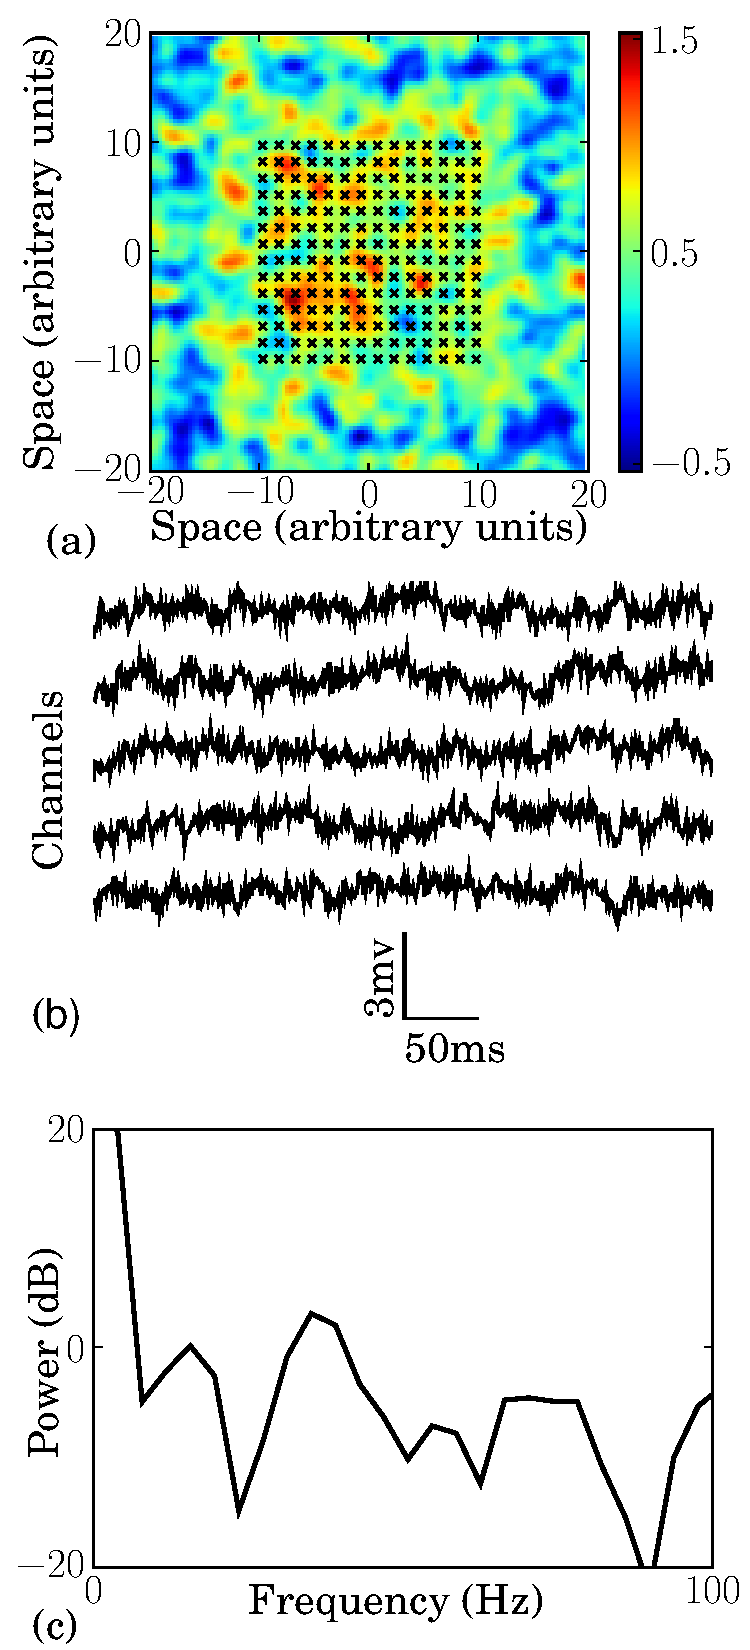
\includegraphics[width=0.3\textwidth]{./Graph/ExperimentFigurePy_1.pdf} 
   	\end{center}
   	\caption{Example of experimental design and model output. \textbf{a}. Example of the neural field with sensors. The centres of the sensors are shown by crosses. \textbf{b} Example of data generated by the model through a subset of the observations. \textbf{c}. Power spectral density of the data generated by an observation showing the typical $1/f$ characteristic of iEEG.} 
   \end{figure}
% \begin{figure}[th]\label{fig:experimental design}
% \begin{center}
% \subfigure[][]{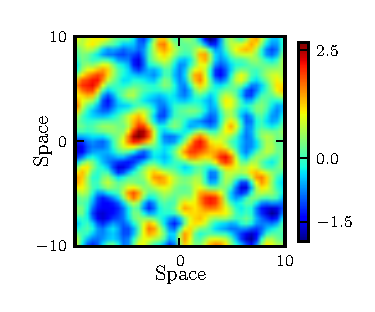
\includegraphics[width=0.35\textwidth]{./Graph/ExperimentFigurePy.pdf}}\\
% \subfigure[][]{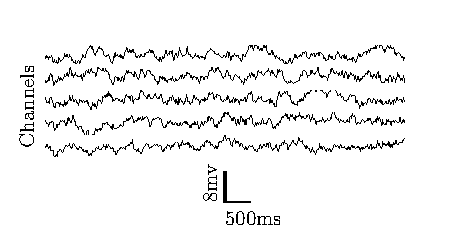
\includegraphics[width=0.35\textwidth]{./Graph/ExperimentFigureEEGPy.pdf}}\\
% \subfigure[][]{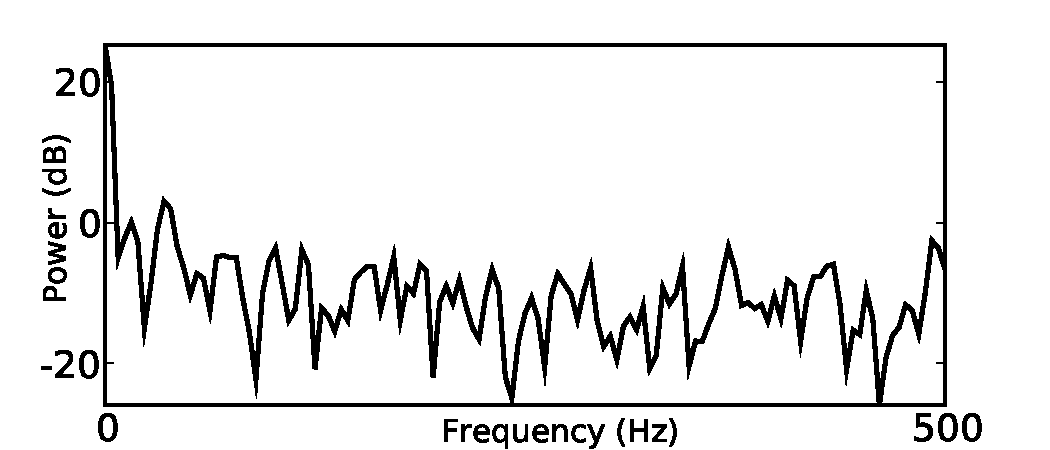
\includegraphics[width=0.35\textwidth]{./Graph/ExperimentFigurePSDPy.pdf}}
% \end{center}
% \caption{Example of experimental design and model output. \textbf{a}. Example of the neural field with sensors. The centres of the sensors are shown by crossed and the sensor widths ($1/2$ height of Gaussian) are shown by the circles. \textbf{b} Example of data generated by the model through the observations. \textbf{c}. Power spectral density of the data generated by an observation showing the typical $1/f$ characteristic of iEEG.} 
% \end{figure}
\begin{figure}[th]
\subfigure[][]{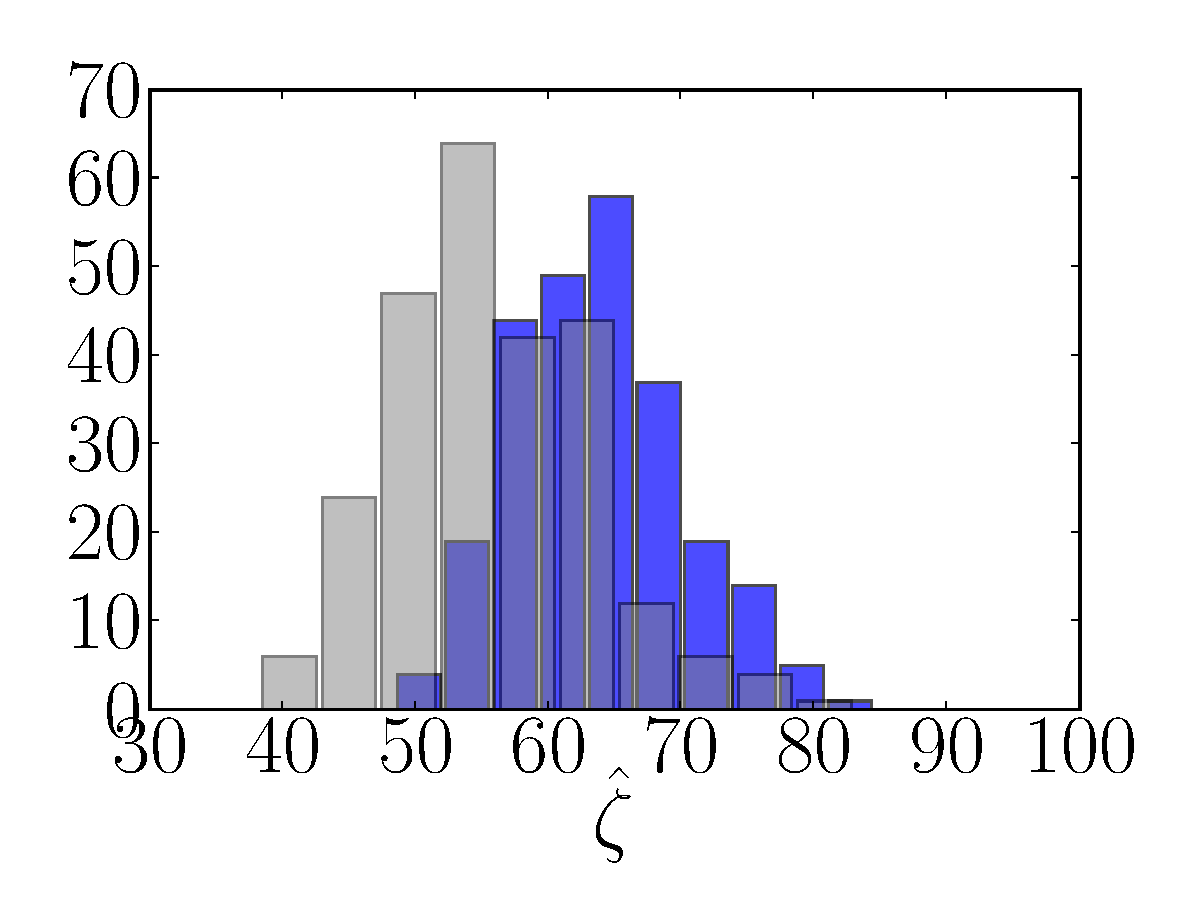
\includegraphics{./Graph/zeta.pdf}}
\subfigure[][]{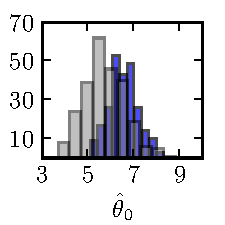
\includegraphics{./Graph/theta0.pdf}}\\
\subfigure[][]{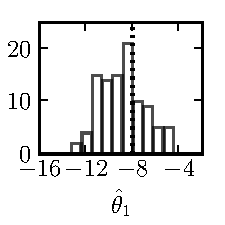
\includegraphics{./Graph/theta1.pdf}}
\subfigure[][]{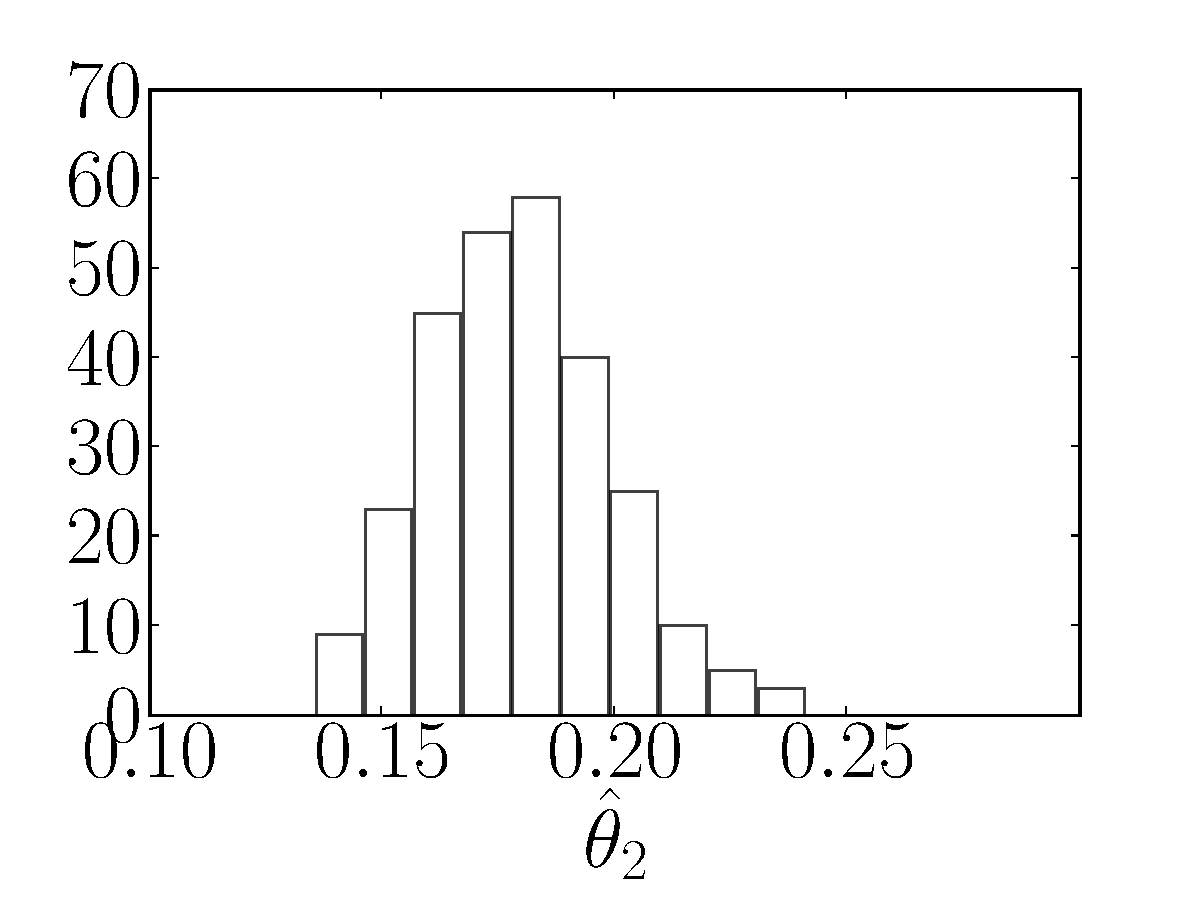
\includegraphics{./Graph/theta2.pdf}}
\caption{Distribution of the parameters estimates over 250
realisations. Grey bars show distributions with wider basis functions ($\sigma_{\phi} = ?$) and blue bars show improved parameter distributions with narrower basis functions ($\sigma_{\phi} = ?$). \textbf{a.} The distribution of the synaptic time constant estimates (true parameter: $\zeta=100$). \textbf{b.} The distribution of the central excitatory connectivity kernel basis function parameters estimates (true parameter: $\theta_0 = 10$). \textbf{c.} The distribution of the surround inhibition connectivity kernel basis function parameter estimates (true parameter: $\theta_1 = -8$). \textbf{d.} The distribution of the longer range excitatory connectivity kernel basis function parameter estimates (true parameter $\theta_3 = 0.5$).}
\label{fig:Parameters}
\end{figure}
\begin{figure}[th]
\subfigure[$\zeta$ convergence]{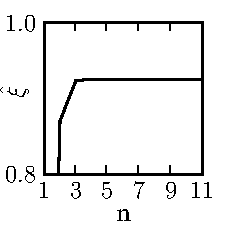
\includegraphics[width=1.5in]{./Graph/ZetaConvergence.pdf}}
\subfigure[][]{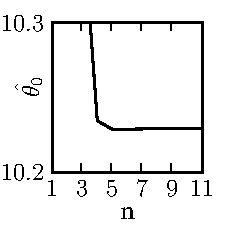
\includegraphics[width=0.24\textwidth]{./Graph/theta0Convergence.pdf}}\\
\subfigure[][]{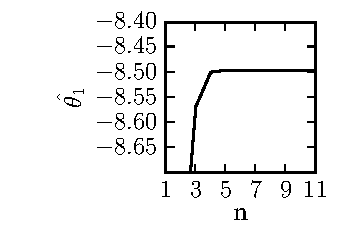
\includegraphics[width=0.24\textwidth]{./Graph/theta1Convergence.pdf}}
\subfigure[][]{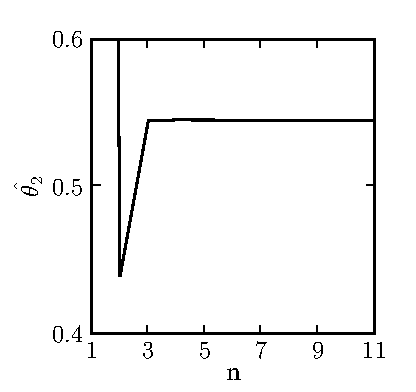
\includegraphics[width=0.24\textwidth]{./Graph/theta2Convergence.pdf}}
\caption{Convergence of the parameters averaged over 250 runs. }
\label{fig:ParametersConvergence}
\end{figure}
\subsection{Spatial Frequency Analysis} 
Using the model selection techniques described in Section~\ref{SpectralAnalysisSection}, the spatial frequency of the field was used to confirm that the spacing and width of the sensors was adequate to capture the significant dynamics of the field. Figure~\ref{fig:FieldFFT}(a) shows the spatial frequency of the field. The cut-off frequency, $\nu_c$, was taken to be \dean{??} ($-3$~dB point). From equation~\ref{eq:MinimumSensorDistance}, this yielded a minimum sensor separation of \dean{??}. This confirms our separation of \dean{??} was enough to prevent problems associated with aliasing.

The spatial frequency of the observations is shown in Figure~\ref{fig:FreqAnalysis}(c). The peak power of the spatial frequency of the observations was approximately \dean{$??$}~dB. The cut-off frequency (-3~dB point) was taken to correspond to  approximately \dean{$??$}~dB. This provided a conservative estimate of the spatial bandwidth. The oversampling parameter $\rho_b$ was set to \dean{??} giving a minimum distance between basis functions of \dean{??} to satisfy Shannon's sampling criterion (from equation~\ref{eq:BasisFunctionSeparation}). The width of the basis functions was chosen such that the basis functions had sufficient overlap to represent the dynamic field. Equation~\ref{eq:WidthCutOffRelationship} (where $sigma_{\phi}^2 = $ \dean{??}) was used to confirm the width of the basis functions was sufficiently small to capture the characteristics of the field.

\begin{figure}
	\label{fig:FreqAnalysis} 
	\begin{center}
\subfigure[][]{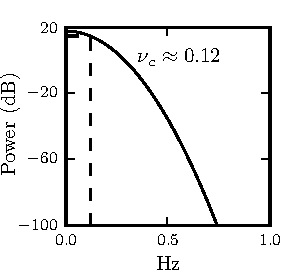
\includegraphics[scale=0.8]{./Graph/BasisChar.pdf}}
\subfigure[][]{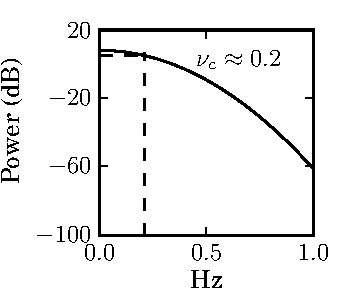
\includegraphics[scale=0.8]{./Graph/SensorChar.pdf}}
\subfigure[][]{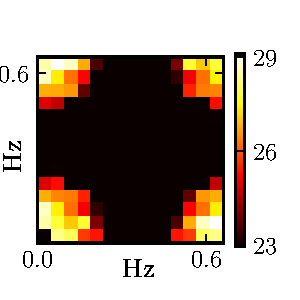
\includegraphics[width=1.8in]{./Graph/ObservationFrequencyResponse.pdf}}\\
	\end{center}
	\caption{Frequency analysis of the. \textbf{a.} The spatial frequency response of a 1-dimensional neural field basis functions project. The symmetry of the field basis functions, connectivity kernel basis functions and sensors allow for the 1-dimensional representation of the spectral characteristics. The dashed line shows the cut-off frequency (-3 dB point). \textbf{b} The spatial frequency response of a 1-dimensional model sensor. The dashed line shows the cut-off frequency (-3 dB point), indicating a wider bandwidth than the field basis function. \textbf{c.} Two 2-dimensional spatial frequency (in power dB, averaged over 200 time steps) of the observed field.} 
\end{figure}
Following this, the distance between basis function, $\Delta_{phi}$, was set to $2.5$ and the basis function width, $\sigma_{\phi}^2$, was set to 3.6, 3.16 mm full width at half maximum. \mike{Analysis said 3.9 from Parham's derivation, but 3.6 still overlaps and allows more high frequency details to be represented.}

\subsection{State and Parameter Estimates} 
\label{sec:state_and_param_results}
To demonstrate the performance of the parameter and state estimation, $250$ realisations of the data were generated. Each realisation consisted of 200~ms of data and the estimation was applied to the final 195~ms, allowing the model to stabilise.\dean{transient!} The initial state and parameters were unknown to the estimator. The distribution of the parameters and the resulting kernel are shown in figure~\ref{fig:Parameters} and figure~\ref{fig:KernelEstimates}, respectively. Although a wide distribution can be seen over the parameter estimates, the ratio between them remains within a narrow range as shown in figure~\ref{fig:ParametersRatio}. The state estimates for one realisation were evaluated by comparing the field reconstruction to the true field using the mean over time of the Root Mean Square Error (RMSE) and standard deviation of the RMSE giving $0.19\pm 0.01$. The RMSE of the field estimate over time is also shown in figure~\ref{fig:RMSE}. A snapshot of the true field, the estimated field and their corresponding error is illustrated in Figure~\ref{fig:FieldEstimate}.

\begin{figure*}
\subfigure[][]{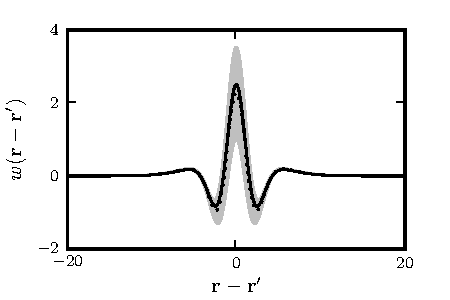
\includegraphics{./Graph/KernelEstimate.pdf}}
\subfigure[][]{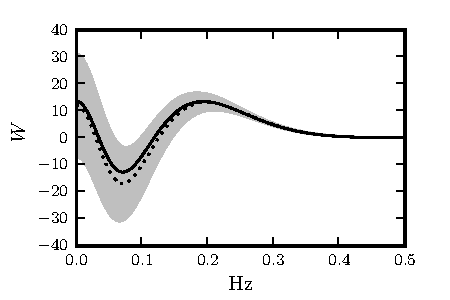
\includegraphics{./Graph/KernelEstimateFFT.pdf}}\\
\caption{Results for connectivity estimate. In all the subplots the true kernel is shown by the solid line, the mean kernel estimate (over 100 realisations) is shown by the dashed line and the 95~\% confidence interval is shown by the shaded grey region. \textbf{a.} Comparison of kernel estimates to true kernel in the spatial domain. \textbf{b.} Comparison of the true kernel to the estimated kernel in the frequency domain. \dean{Note: needs to be changed to absolute values if we include it.} \dean{Note: Power and dB needs to be non-italicised.}}
\label{fig:KernelEstimates}
\end{figure*}
\begin{figure}[th]
\subfigure[][]{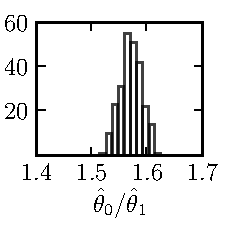
\includegraphics{./Graph/theta0_theta1_ratio.pdf}}
\subfigure[][]{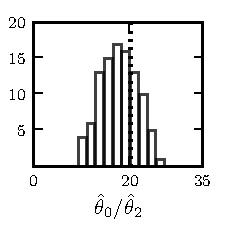
\includegraphics{./Graph/theta0_theta2_ratio.pdf}}\\
\caption{Distribution of the connectivity kernel basis function parameter ratios over 250 realisations. \textbf{a.} The absolute value of the ratio of the local excitatory parameter to the surround inhibition parameter (true ratio is 1.25). \textbf{b.} The ratio of the local excitatory parameter to the longer range excitatory parameter (true ratio is 20).}
\end{figure}
\label{fig:ParametersRatio}
\begin{figure}[th]
\centering
\subfigure[][]{\label{fig:FieldFFT}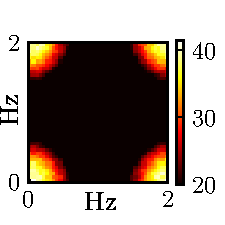
\includegraphics[scale=0.9]{./Graph/FFTTrueField.pdf}}
\subfigure[][]{\label{fig:EstimatedFieldFFT}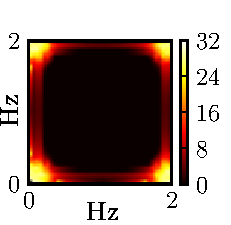
\includegraphics[scale=0.9]{./Graph/FFTEstimatedField.pdf}}\\
\caption{Spatial frequency of the neural fields. \textbf{a.} The average (over time) spatial frequency of the neural field. \textbf{b.} The average (over time) spatial frequency of the estimated neural field resulting from the basis function decomposition. As a result of the band limiting properties of the sensors and basis functions the reconstructed shows a narrower bandwidth.}
\label{fig:FFTTrueEstimate}
\end{figure}

  \begin{figure}
   	\begin{center}
   		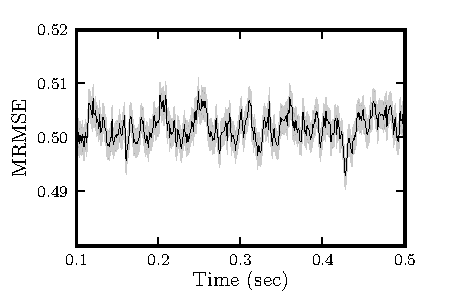
\includegraphics{./Graph/MRMSE.pdf} 
   	\end{center}
   	\caption{The mean of average RMSE of the estimated field over 250 realisations (solid line) and the 95~\% confidence interval (grey region). \dean{David suggested for us to use percentage error, and use a hard threshold of points close to zero to stop problems with divide by zeros. Also, it might be good to show the data points along the line, so we can see the number of iterations it takes to stabilise.}} 
\label{fig:RMSE}
   \end{figure}
\begin{figure*}[!th]
\centering 
\subfigure[][]{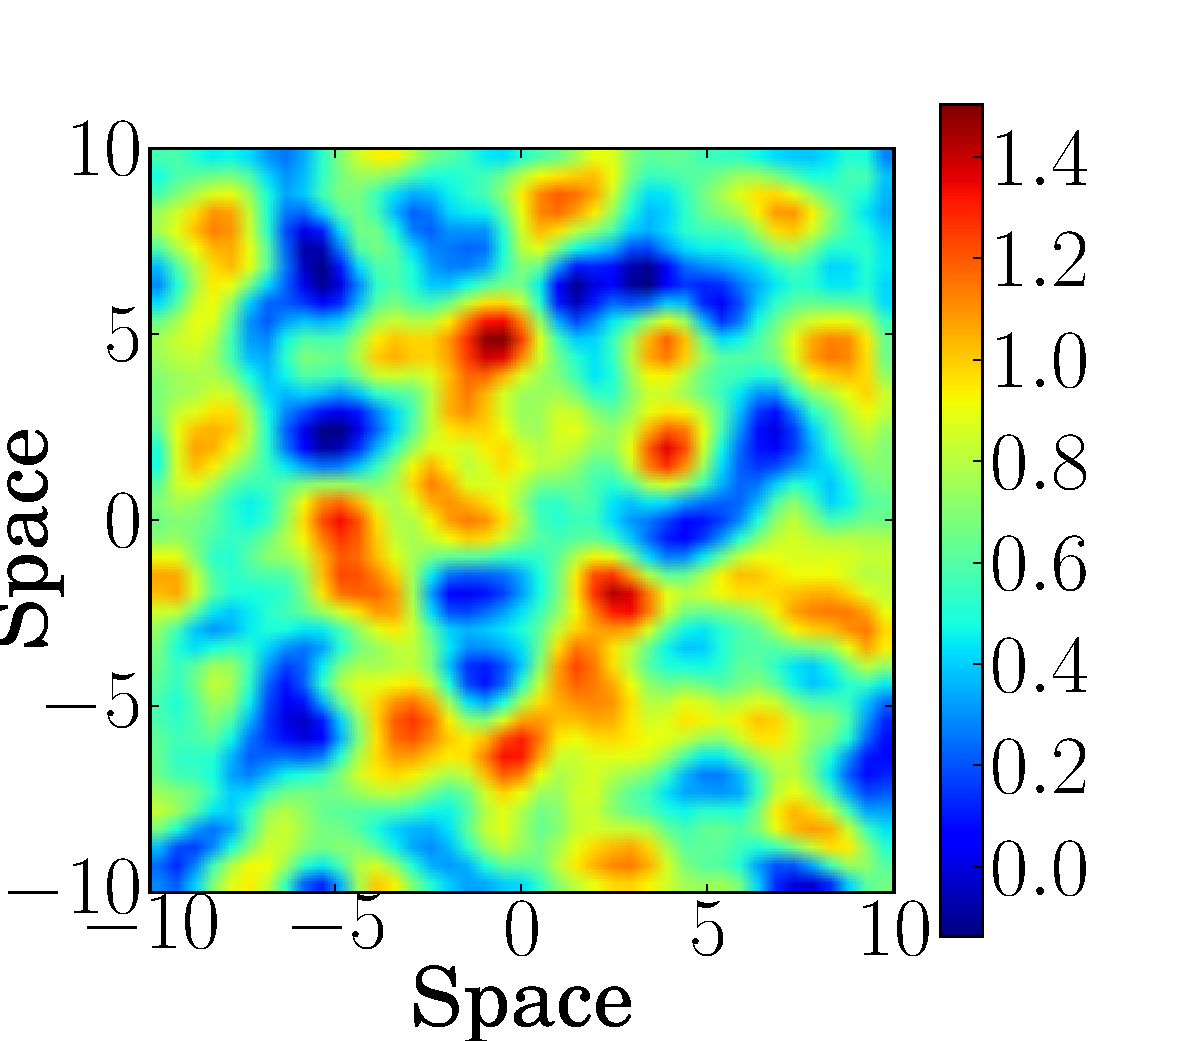
\includegraphics[scale=0.8]{./Graph/TrueField90.pdf}}
\subfigure[][]{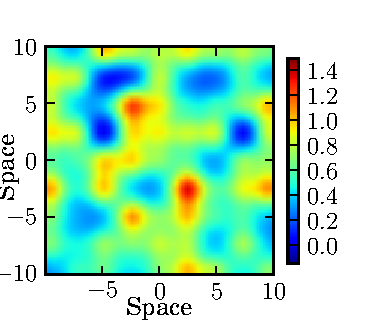
\includegraphics[scale=0.8]{./Graph/EstimatedField90.pdf}}
\subfigure[][]{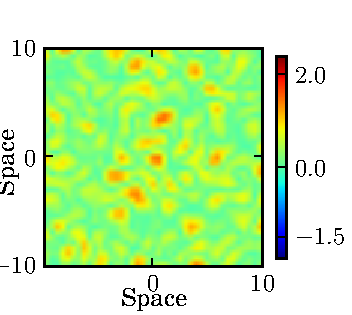
\includegraphics[scale=0.8]{./Graph/EstimationError90.pdf}}\\
\caption{Examples of the neural fields. \textbf{a.} The true field from the non-reduced model the was used to generate data. \textbf{b.} The reconstructed estimated field of the reduced model. \textbf{c.} The absolute error between the true and reconstructed fields.}
\label{fig:FieldEstimate}
\end{figure*}

\section{Discussion}\label{DiscussionSection}

\dean{NOTE: I HAVE ADDED A SENTENCE DESCRIBING SIMPLY WHAT I WANT TO SAY IN EACH PARAGRAPH. PLEASE USE THIS AS A GUIDE FOR EDITING.}

POSSIBLE SOURCES OF THE ERROR
\begin{itemize}
	\item slope of nonlinearity interacting with tails of Gaussian basis functions
	\item loss of high frequency info from basis function decomposition
	\item distortions of the spectral content of the basis function from the nonlinearity
	\item disturbance covariance too narrow
	\item disturbance variance too low (not exciting the kernel enough)
	\item boundary conditions
	\item
\end{itemize}

\dean{FIRST DESCRIBE AN OVER ALL SUMMARY OF WHAT WE HAVE DONE AND WHAT IS NOVEL}
This paper presents a novel framework for model reduction to facilitate practical state and parameter estimation of spatio-temporal neural fields. A basis function decomposition reduces the infinite dimensional neural field (continuous space), to a finite dimensional state-space model. The level of detail of the estimated field is related to the basis functions decomposition, providing a flexible framework where a trade-off can be made between physiological detail and computational complexity. Using the state-space model, the unscented Rauch Tung Striebel Smoother was applied for state estimation. Using the sequence of state estimates, a least squares algorithm was implemented for parameter estimation.  

\dean{DISCUSS RESULTS: FREQ ANALYSIS. USE THIS TO JUSTIFY KERNEL ERRORS.}
The frequency analysis and model selection tools presented in this paper specify the sensor and field basis function arrangement required to form a state-space model that is capable of capturing the dominant cortical dynamics. In addition to providing conditions to ensure the reduced model can capture the significant spectral properties of the field, these tools can be used to better design electrophysiological recording techniques avoid spatial aliasing. The effect of the basis function decomposition will restrict the frequency content of the estimated field. This is evident in when comparing figures~\ref{fig:FieldFFT} and~\ref{fig:EstimatedFieldFFT} where the estimated field is spatially band-limited. The spatial frequency content of the field is governed by disturbance covariance and the shape of the connectivity kernel. Therefore some information will be lost due to the field decomposition. The implication of this loss of information is the high spatial frequency content of the connectivity kernel. This is demonstrated in figure~\ref{fig:KernelEstimates} where the frequency content of the estimated connectivity kernel is less than the true kernel.

\dean{DISCUSS THAT EVEN THOUGH THE KERNEL ESTIMATE IS NOT EXACT, IT IS USEFUL TO KNOW THE RATIO OF EXCITATION TO INHIBITION AND THAT RELATIVE MEASURES CAN BE ACCURATELY TRACKED}
Even though the some high spatial frequency content of the connectivity kernel is lost through the basis function decomposition, the dominant dynamics are still captured with the estimated reduced model. This is illustrated in figure~\ref{fig:FieldEstimate}. In addition, the ratio of the kernel parameters follows a tight distribution as seen in figure~\ref{fig:ParametersRatio}. This indicates that the ratio of excitation to inhibition can be tracked with this approach. 

\dean{NEED TO ADD SOMETHING ABOUT THE TIME CONSTANT }

\dean{DISCUSS THE IMPLICATION OF ESTIMATING INTRACORTICAL CONNECTIVITY AND WHERE WE FIT WITHIN OTHER FUNCTIONAL CONNECTIVITY RESEARCH AREAS}
To the authors' best knowledge, this is the first paper to propose an estimation framework for intracortical connectivity from electrophysiological data. The importance of the estimation framework can be illustrated by considering that the connectivity structure at this scale can not be estimated using diffusion tensor imaging due to the near isotropic diffusion of water in grey matter~\cite{Assaf2008}. In addition, other non-model-based techniques for estimating functional connectivity, such as Granger causality~\cite{Hesse2003}, the direct transfer function~\cite{Kaminski1991} and partial directed coherence~\cite{Sameshima1999}, are restricted to the spatial scales of the recording electrodes. The model-based technique proposed in this paper estimates the connectivity structure of the number of sensors. An advantage of the auto-regressive (AR) methods is that they allow for anisotropic connectivity, which is present in cortico-cortical fibres. It should be noted, however, that the AR and the proposed model-based methods are complementary, where connectivity is estimated at different spatial scales. Therefore, we envisage that by combining these methods a more realistic model can be acquired. A recent theoretical study~\cite{Jirsa2009} has demonstrated the importance of this multi-scale structure in generating the characteristic rhythms of the brain.

\dean{DISCUSS A BIG PICTURE. WHERE THIS WORK SHOULD GO AND WHERE IT SHOULD BE APPLIED IN THE FUTURE}
Generating patient specific neural field models has the potential to have significant impact on several areas of neuroscientific research and clinical neurology. Specifically, the development of a patient-specific state-space model will allow for the application of systems theoretical techniques from engineering to be applied to neuro-dynamics. For example, state tracking could be used in brain-computer interface or epileptic seizure prediction applications, where specific regions of the state-space may indicate intent of movement or imminent seizures. Recent studies using neural field models have demonstrated the theoretical implications of specific connectivity structure of the cortical columns in neural field models, where the connectivity kernel governs where a Turing-Hopf bifurcation occurs~\cite{Hutt2005}, and the types of oscillations that can be generated~\cite{Schmidt2009}. This implies that if we can estimate the connectivity structure for an individual, then we could capture patient specific neurodynamics that lead to hyper-synchronous oscillatory states such as Turing patterns. In addition, a patient specific state-space model will allow application of control engineering techniques to robustly prevent the neuro-dynamics entering pathological regions of state-space using electrical stimulation. 

Parameter estimation may also have significant impact on the treatment of disease. For example, recent theoretical work has demonstrated that seemingly similar electrographic seizures in absence epilepsy may arise from abnormal excitatory or inhibitory mechanisms~\cite{Marten2009}. These very different mechanisms would require very different medications for successful treatment. However, the underlying mechanisms would be hidden from the clinician in the normal clinical setting. Successful parameter estimation has the potential to reveal these hidden mechanisms allowing for improved treatment strategies.

\dean{DISCUSS HOW IT CAN LINK THEORETICAL MODELLING STUDIES TO DATA.}
This estimation framework also has theoretical implications by establishing a framework that has the potential to allow testing of hypotheses that have been generated in theoretical studies and to validate neural field models. For example, it has been hypothesised that so-called ``bump solutions'' are a possible mechanism for short term memory formation~\cite{Coombes2005}. Using the proposed model-based framework, we can reconstruct a neural field from data, and estimate parameters and check if they correspond the the theoretically derived parameters where these bump solutions can exist. In addition, the parameters and the state-space can be explored during other cognitive tasks and states of arousal such as during sleep and under anaesthesia. 

\dean{DISCUSS SHORT-COMINGS AND FUTURE WORK}
In this paper, the widths of the connectivity kernel basis functions are assumed to be known. In future work, we plan to extend this work to estimate the connectivity structure width unknown kernel basis function widths. We hope to achieve this by using a sufficiently large set of connectivity basis functions within the physiological plausible limits, and allow the estimation procedure take care of the weights. In addition, we plan to show in future work how the assumption of homogeneity can be relaxed, where heterogeneity can be modelled by careful placement of field basis functions. For example, if cortical regions have a greater density of neural populations, then more basis functions can be used in these areas. In this scenario, model selection and basis function positioning can be achieved using instantaneous frequency analysis of the the neural field or alternative model selection tools based on information criteria. Future work should also be targeted to include a more realistic synaptic response kernel, with finite rise and decay times and finite propagation times into the neural field equations.

\begin{itemize}
	\item What about the transient! The need for activity to perform estimation. \dean{To Learn You Must Perturb!} 
\end{itemize}
% 
% \section{Conclusion}\label{ConclusionSection}
% This paper presented a novel model-based framework for patient-specific state and parameter estimation of neural fields. This framework enables a fundamental link between patient-specific physiologic data and theoretical neural field models. This link has the potential to lead to advances in our basic understanding of the dynamics of the brain at the macro/mesoscopic scale. Forming a greater understanding neural dynamics at this scale may lead to new and improved treatment options for diseases such as epilepsy.

\appendix 
\section{Discrete Time Model}\label{Time Discretization} To form the IDE neural field model a time discretisation must be perform. We used a one-step Euler method where Eq.~\ref{FinalFormContinuous} can be approximated by 
\begin{eqnarray}
	\label{Euler Approximation} \lefteqn{\frac{v\left( \mathbf{r},t+T \right) - v\left( \mathbf{r},t\right)}{T_s} =}\nonumber\\
& -&\zeta v\left( \mathbf{r},t \right) + \int_\Omega {w\left( \mathbf{r}-\mathbf{r}' \right)f\left( {v\left( \mathbf{r}',t \right)} \right)d\mathbf{r}'}.\nonumber \\ 
\end{eqnarray}
For clarity, we shall index time points in the discrete time form of the model using the subscript $t$ and the next time point as $t+1$. Rearranging Eq.~\ref{Euler Approximation} we get 
\begin{eqnarray}
	\label{Euler Approximation2} v_{t+1}\left( \mathbf{r}\right) &=& v_t\left( \mathbf{r}\right) -T_s \zeta v_t\left( \mathbf{r}\right)\nonumber \\
&+& T_s \int_\Omega {w\left( \mathbf{r}-\mathbf{r}' \right)f\left( {v_t\left( \mathbf{r}'\right)} \right)d\mathbf{r}'}.\nonumber \\ 
\end{eqnarray}
The discrete time form of the model is 
\begin{equation}
	\label{Discrete Time Model1} v_{t+1}\left(\mathbf{r}\right) = \xi v_t\left(\mathbf{r}\right) + T_s \int_\Omega { w\left(\mathbf{r}-\mathbf{r}'\right) f\left(v_t\left(\mathbf{r}'\right)\right) d\mathbf{r}'}, 
\end{equation}
where $\xi = 1 - T_s \zeta$. 
\section{Numerical Simulation of IDE Model}\label{Space Discretization} To solve the intregro-difference equation in Eq.~\ref{Discrete Time Model1} we define the spatial aspect of the model on a regular square $i,j$ grid of neural masses, where the spatial step size $\Delta \mathbf{r}_i = \Delta \mathbf{r}_j = \Delta $ giving 
\begin{eqnarray}
	\label{discrete space} \lefteqn{v_{t+1}\left(\mathbf{r}_{ij}\right)=}\nonumber\\
&&\xi v_t\left(\mathbf{r}_{ij}\right)+T_s \Delta^2\sum_{i=1}^{i=I}{\sum_{j=1}^{j=J}{w\left(\mathbf{r}-\mathbf{r}_{ij}'\right)f\left( v_t\left( \mathbf{r}_{ij}'\right)\right)}}\nonumber\\
&+& e_t(\mathbf{r}_{i,j}), 
\end{eqnarray}
where $e_t(\mathbf{r}_{i,j}) \sim \mathcal{N}\left(0,\Sigma\right)$. We have used free boundary conditions and extended the spatial domain to alleviate problems associated with edge effects. 
% \section{Reduction to Finite State-Space Model}\label{Simplifying Decomposition} 
% Starting from equation~\ref{reduced continuous model} we multiply throughout by $\boldsymbol{\phi}(r)$ and integrate over the spatial domain $\Omega$ to get 
% \begin{eqnarray}
% 	\label{StartofReduction}\lefteqn{ \int_\Omega {\boldsymbol{\phi} \left(\mathbf{r}\right)\boldsymbol{\phi}^{\top}\left(\mathbf{r}\right) d\mathbf{r}} \mathbf{x}_{t+1}=} \nonumber\\
%  &&T_s \int_\Omega {\boldsymbol{\phi} (\mathbf{r}) \boldsymbol{\theta}^{\top} \int_\Omega {\boldsymbol{\psi} \left(\mathbf{r}-\mathbf{r}'\right) f\left(\boldsymbol{\phi}^{\top}\left(\mathbf{r}'\right) \mathbf{x}_t \right)d\mathbf{r}'}d\mathbf{r}} \nonumber\\
% &+& \xi\int_\Omega {\boldsymbol{\phi}(\mathbf{r})\boldsymbol{\phi}^{\top}(\mathbf{r})d\mathbf{r}} \mathbf{x}_t+
% \int_\Omega{\boldsymbol{\phi} \left(\mathbf{r}\right) e_t\left(\mathbf{r}\right)d\mathbf{r}}. 
% \end{eqnarray}
% Now defining
% \begin{equation}\label{eq:DefGamma2}
% 	\boldsymbol{\Gamma} = \int_\Omega {\boldsymbol{\phi} \left(\mathbf{r}\right)\boldsymbol{\phi} ^{\top}\left(\mathbf{r}\right)d\mathbf{r}}, 
% \end{equation}
% and substituting equation~\ref{eq:DefGamma2} into equation~\ref{StartofReduction} and cross-multiplying by $\boldsymbol{\Gamma}^{-1}$ gives 
% \begin{eqnarray}\label{eq:ReducedForm}
% 	 \lefteqn{\mathbf{x}_{t+1} \nonumber = T_s\boldsymbol{\Gamma}^{ - 1}\int_\Omega {\boldsymbol{\phi}(\mathbf{r}) \int_\Omega {f(\boldsymbol{\phi}^{\top}(\mathbf{r}')\mathbf{x}_t) \boldsymbol{\psi}^{\top} (\mathbf{r}-\mathbf{r}')d\mathbf{r}'} d\mathbf{r}} \boldsymbol{\theta}} \nonumber\\
% &+&\xi\mathbf{x}_t + \boldsymbol{\Gamma}^{-1} \int_\Omega{\boldsymbol{\phi}(\mathbf{r})e_t(\mathbf{r})d\mathbf{r}}.
% \end{eqnarray}
% Equation~\ref{eq:ReducedForm} can be simplified by exploiting the symmetry (isotropy) of the connectivity kernel where
% \begin{equation}
% 	\boldsymbol{\psi} (\mathbf{r}-\mathbf{r}') = \boldsymbol{\psi} (\mathbf{r}'-\mathbf{r}).
% \end{equation}
% To make the simplification we first define
% \begin{equation}\label{eq:DefPsi}
% 	\boldsymbol{\Psi}(\mathbf{r}') = T_s\boldsymbol{\Gamma}^{-1}\int_\Omega {\boldsymbol{\phi}(\mathbf{r})\boldsymbol{\psi} (\mathbf{r}'-\mathbf{r})d\mathbf{r}},
% \end{equation}
% which is constant and can be defined analytically. Now substituting~\ref{eq:DefPsi} into~\ref{eq:ReducedForm} gives
% \begin{equation}
% 	\mathbf{x}_{t+1} \nonumber = \int_\Omega \boldsymbol{\Psi}(\mathbf{r}') f(\boldsymbol{\phi}^{\top}(\mathbf{r}')\mathbf{x}_t) d\mathbf{r}' \boldsymbol{\theta} + \xi\mathbf{x}_t + \boldsymbol{\Gamma}^{-1} \int_\Omega{\boldsymbol{\phi}(\mathbf{r})e_t(\mathbf{r})d\mathbf{r}}.
% \end{equation}
% \dean{DEFINE q HERE!!!!!}
\section{}\label{ColoredNoise} 
\newtheorem{lemma}{Lemma} 
\begin{lemma}
	Consider the i.i.d. noise term $e_t(\mathbf{r})\sim\mathcal{GP}(\mathbf 0,\gamma(\mathbf{r}-\mathbf{r'}))$ then 
	\begin{equation}\label{eq:AppendixWt} 
		\mathbf e_t=\boldsymbol{\Gamma}^{-1}\int_\Omega {\boldsymbol{\phi} ( \mathbf{r} )e_t( \mathbf{r} )d\mathbf{r}} 
	\end{equation}
	is a vector valued, zero mean normally distributed white noise process with covariance 
	\begin{equation}
		\boldsymbol\Sigma_e =\mathbf{\Gamma}^{-1}\int_{\Omega}\int_{\Omega}\boldsymbol{\phi}\left(\mathbf r\right) \gamma\left(\mathbf r- \mathbf r' \right)\boldsymbol{\phi}\left(\mathbf r'\right)^{\top}d\mathbf r' d\mathbf r\mathbf{\Gamma}^{- \top} 
	\end{equation}
	\label{lemma:FieldCovariance} 
\end{lemma}
\section*{Proof} Equation (\ref{eq:AppendixWt}) is a linear function of $e_t(\mathbf r)$ and hence $\mathbf{e}_t$ is also normally distributed. The expected value of $\mathbf e_t$ is given by 
\begin{eqnarray}
	\mathbf E\left[ \mathbf e_t\right]&=& \mathbf{\Gamma}^{-1}\int_{\Omega}\boldsymbol\phi\left(\mathbf{r}\right)\mathbf E\left[e_t\left(\mathbf{r}\right)\right] d\mathbf{r} \nonumber \\
	&=&\mathbf 0 
\end{eqnarray}
The covariance of $\mathbf{e}_t$ is 
\begin{eqnarray}
	\lefteqn{\mathbf{\Sigma}_e} \nonumber \\ 
&=&\mathbf{\Gamma}^{-1}\mathbf E[\int_{\Omega}\boldsymbol{\phi}(\mathbf{r})e_t(\mathbf{r})d\mathbf{r} \int_{\Omega}\boldsymbol{\phi}^{\top}(\mathbf{r}') e_t(\mathbf{r}')d\mathbf{r}']\mathbf{\Gamma}^{- \top} \nonumber \\
	&=&\mathbf{\Gamma}^{-1}\int_{\Omega}\int_{\Omega} \boldsymbol{\phi}(\mathbf{r}) \mathbf E[e_t(\mathbf{r})e_t(\mathbf{r}')]\boldsymbol{\phi}^{\top}(\mathbf{r}')d\mathbf{r}' d\mathbf r\mathbf{\Gamma}^{- \top} \nonumber\\
	&=&\mathbf{\Gamma}^{-1}\int_{\Omega}\int_{\Omega}\boldsymbol{\phi}(\mathbf r) \gamma(\mathbf r- \mathbf r' )\boldsymbol{\phi}^{\top}(\mathbf r')d\mathbf r' d\mathbf r\mathbf{\Gamma}^{-\top} 
\end{eqnarray}
\section{Proof of \ref{eq:GaussianFT} and \ref{eq:WidthFrequencyRelationship} }\label{ap:FrequencyAnalysis}
Applying the \textit{n}-dimensional Fourier transform \cite{Arsac1966} to an \textit{n}-dimensional Gaussian centered at the origin yields
\begin{eqnarray}\label{eq:AppendixGaussianFT}
 \lefteqn{\boldsymbol\Phi(\boldsymbol \nu)=\int_{\mathcal R^n}\mathrm{exp}({-\frac{1}{\sigma_{\phi}^2}\mathbf r^\top\mathbf r})\mathrm{exp}(-2\pi i\boldsymbol\nu^\top\mathbf r)d\mathbf r} \nonumber \\
&=&\int_{\mathcal R^n}\mathrm{exp}(-\frac{1}{\sigma_{\phi}^2}\left[\mathbf r +\sigma_{\phi}\pi i \boldsymbol\nu\right]^\top\left[\mathbf r +\sigma_{\phi}\pi i \boldsymbol\nu\right])d\mathbf r \nonumber \\
&\times& \mathrm{exp}(-\sigma_{\phi}^2\pi^2\boldsymbol\nu^\top \boldsymbol\nu)
\end{eqnarray}
where 
\begin{eqnarray}\label{eq:IntegralOfGaussian}
\int_{\mathcal R^n}\mathrm{exp}(-\frac{1}{\sigma_{\phi}^2}\left[\mathbf r +\sigma_{\phi}\pi i \boldsymbol\nu\right]^\top\left[\mathbf r +\sigma_{\phi}\pi i \boldsymbol\nu\right])d\mathbf r&& \nonumber \\
=(\pi\sigma_{\phi}^2)^{\frac{n}{2}}&&
\end{eqnarray}
substituting \ref{eq:IntegralOfGaussian} in \ref{eq:AppendixGaussianFT} gives another scaled  Gaussian 
\begin{equation}
   \boldsymbol\Phi(\boldsymbol\nu)=(\pi\sigma_{\phi}^2)^{\frac{n}{2}}\mathrm{exp}(-\sigma_{\phi}^2\pi^2\boldsymbol\nu^\top \boldsymbol\nu)
\end{equation}
substituting $\sigma_{\nu}^2=\frac{1}{\pi^2\sigma_{\phi}^2}$ gives 
\begin{equation}
\boldsymbol\Phi(\boldsymbol \nu)=(\frac{1}{\pi\sigma_{\nu}^2})^{\frac{n}{2}}\mathrm{exp}(-\frac{1}{\sigma_{\nu}^2}\boldsymbol\nu^\top \boldsymbol\nu).
\end{equation}
and hence completing the proof. For 3 dB attenuation at $\boldsymbol\nu_c$ we need to set
\begin{eqnarray}
 |\boldsymbol\Phi(\boldsymbol\nu_c)|^2=\frac{1}{2}|\boldsymbol\Phi(\mathbf 0)|^2
\end{eqnarray}
%\left(\frac{1}{\pi\sigma_{\nu}^2}\right)^{n}\mathrm{exp}\left(-\frac{2}{\sigma_{\nu}^2}\boldsymbol\nu_c^\top \boldsymbol\nu_c\right)\\
solving for $\sigma_{\nu}^2$ we get
\begin{equation}
 \sigma_{\nu}^2=\frac{2\boldsymbol\nu_c^\top \boldsymbol\nu_c}{\ln 2 }.
\end{equation}

\section{Parameter Estimation Using Least Squares}\label{LeastSquaresAppendix} 
The finite state space model  given in \ref{eq:ReducedForm} is linear in parameters and therefore Least Square (LS) method can be applied to estimate the unknown parameters. We define $L \times n_{\theta}$ matrix
\begin{eqnarray}\label{eq:QMatrix}
	\lefteqn {\mathbf{Q}(\mathbf{x}_t)=} \\
&&\boldsymbol{\Gamma}^{ - 1}\int_\Omega {\boldsymbol{\phi}(\mathbf{r}) \int_\Omega {f(\boldsymbol{\phi}^{\top}(\mathbf{r}')\mathbf{x}_t)\boldsymbol{\psi}^{\top} \left(\mathbf{r}-\mathbf{r}'\right)d\mathbf{r}'} d\mathbf{r}}\nonumber
\end{eqnarray}
by substituting \ref{eq:Reducednoiseterm} and \ref{eq:QMatrix} in \ref{eq:ReducedForm} and using $\xi = 1-\zeta T_s$ at each time instant we can write
\begin{eqnarray}
	\mathbf x_{1}&=&\mathbf x_{0}+T_s \mathbf Q(\mathbf x_0) \boldsymbol{\theta}-\zeta T_s\mathbf x_0+\mathbf e_0 \nonumber \\
	\mathbf x_{2}&=&\mathbf x_{1}+T_s \mathbf Q(\mathbf x_1) \boldsymbol{\theta}-\zeta T_s\mathbf x_1+\mathbf e_1\nonumber\\
	&\vdots& \\
	\mathbf x_{T}&=&\mathbf x_{T-1}+T_s \mathbf Q(\mathbf x_{T-1}) \boldsymbol{\theta}-\zeta T_s\mathbf x_{T-1}+\mathbf e_{T-1} \nonumber
\end{eqnarray}
% in matrix form 
% \begin{equation}
% 	\left[
% 	\begin{array}{cccc}
% 		\mathbf x_{1}\\\mathbf x_{2}\\\vdots\\\mathbf x_{n}
% 	\end{array}
% 	\right] -\left[
% 	\begin{array}{cccc}
% 		\mathbf x_{0}\\\mathbf x_{1}\\\vdots\\\mathbf x_{n-1}
% 	\end{array}
% 	\right] =T_s\left[
% 	\begin{array}{cc}
% 		\mathbf Q(\mathbf x_0)&-\mathbf x_{0}\\\mathbf Q(\mathbf x_1)&-\mathbf x_{1}\\\vdots\\
% 		\mathbf Q(\mathbf x_{n-1})&-\mathbf x_{n-1}
% 	\end{array}
% 	\right] \left[
% 	\begin{array}{cc}
% 		\boldsymbol{\theta} \\
% 		\zeta
% 	\end{array}
% 	\right]+\left[
% 	\begin{array}{cccc}
% 		\mathbf e_0\\\mathbf e_1\\\vdots\\\mathbf e_{n-1}
% 	\end{array}
% 	\right] 
% \end{equation}
 in compact form we have 
\begin{equation}
	\mathbf Z=\mathbf X \mathbf W+\boldsymbol \xi 
\end{equation}
where 
\begin{small}
\begin{equation*}
	\mathbf Z=\left[
	\begin{array}{cccc}
		\mathbf x_{1}-\mathbf x_{0}\\
		\mathbf x_{2}-\mathbf x_{1}\\\vdots\\
		\mathbf x_{T}-\mathbf x_{T-1}
	\end{array}
	\right],\quad \mathbf X=T_s\left[
	\begin{array}{cccc}
		\mathbf Q(\mathbf x_0)&-\mathbf x_{0}\\
		\mathbf Q(\mathbf x_1)&-\mathbf x_{1}\\\vdots\\
		\mathbf Q(\mathbf x_{T-1})&-\mathbf x_{T-1}
	\end{array}
	\right] 
\end{equation*}
\end{small}
and
\begin{small}
\begin{equation*}
\quad \mathbf W=\left[
	\begin{array}{cc}
		\boldsymbol{\theta} \\
		\zeta
	\end{array}
	\right],\quad \boldsymbol \xi=\left[
	\begin{array}{cccc}
		\mathbf e_0\\\mathbf e_1\\\vdots\\\mathbf e_{n-1}
	\end{array}
	\right] 
\end{equation*}
\end{small}
using the LS method $ \mathbf W$ can be estimated 
\begin{equation}
	\mathbf W\approx(\mathbf X^\top\mathbf X)^{-1}\mathbf X^\top\mathbf Z 
\end{equation}

\section{Parameter Estimation Using Least Squares - Dean}\label{App:LeastSquaresAppendix} 
The finite state space model given in \ref{eq:ReducedForm} is linear with respect to parameters. Therefore a least square (LS) method can be applied to estimate the unknown parameters. The create the least squares parameter estimator we first define the $L \times n_{\theta}$ matrix
\begin{equation}
	\mathbf{q}(\mathbf{x}_t) = \int_\Omega \boldsymbol{\Psi}(\mathbf{r}') f(\boldsymbol{\phi}^{\top}(\mathbf{r}')\mathbf{x}_t) d\mathbf{r}'.
\end{equation}
Now given a state estimate sequence from the unscented Rauch Tung Striebel smoother (URTSS), we can write
\begin{eqnarray}
	\mathbf x_{1} &=& \mathbf{q}(\mathbf x_0) \boldsymbol{\theta}+\xi\mathbf x_0+\mathbf e_0 \nonumber \\
	\mathbf x_{2} &=& \mathbf{q}(\mathbf x_1) \boldsymbol{\theta}+\xi\mathbf x_1+\mathbf e_1 \nonumber \\
	&\vdots& \\
	\mathbf x_{T}&=&\mathbf{q}(\mathbf x_{T-1}) \boldsymbol{\theta}+\xi\mathbf x_{T-1}+\mathbf e_{T-1}. \nonumber \\
\end{eqnarray}
This can be written in the compact form
\begin{equation}
	\mathbf Z=\mathbf X \mathbf W+\mathbf{e} 
\end{equation}
where
\begin{small}
\begin{equation*}
	\mathbf Z=\left[
	\begin{array}{cccc}
		\mathbf x_{1}\\
		\mathbf x_{2}\\
		\vdots\\
		\mathbf x_{T}
	\end{array}
	\right],\quad \mathbf X=\left[
	\begin{array}{cccc}
		\mathbf q(\mathbf x_0)& \mathbf x_{0}\\
		\mathbf q(\mathbf x_1)& \mathbf x_{1}\\
		\vdots & \vdots\\
		\mathbf q(\mathbf x_{T-1})& \mathbf x_{T-1}
	\end{array}
	\right] 
\end{equation*}
\end{small}
and
\begin{small}
\begin{equation*}
\quad \mathbf W=\left[
	\begin{array}{cc}
		\boldsymbol{\theta} \\
		\xi
	\end{array}
	\right],\quad \mathbf{e}=\left[
	\begin{array}{cccc}
		\mathbf e_0\\
		\mathbf e_1\\
		\vdots\\
		\mathbf e_{T-1}
	\end{array}
	\right].
\end{equation*}
\end{small}
Following this, the parameters, $ \mathbf W$, can be estimated by
\begin{equation}
	\mathbf W\approx(\mathbf X^\top\mathbf X)^{-1}\mathbf X^\top\mathbf Z. 
\end{equation}
\section{Parameters} 
\begin{tabular}
	{c|c} Symbol & Description \\
	\hline
	\\ & \textbf{Domain and indicies} \\
	\hline
	$\Omega$ & spatial domain \\
	$t$ & time (seconds) \\
	$\mathbf{r}$ & spatial location \\
	$n$ & sensor index $n=1,..,N$ \\
	$T$ & time step \\
	\\ & \textbf{Spatiotemporal Signals} \\
	\hline
	$y(\mathbf{r}_n,t)$ & observation \\
	$v(\mathbf{r},t)$ & mean membrane potential \\
	$g(\mathbf{r},t)$ & average action potential rate \\
	$f(\mathbf{r},t)$ & firing function rate \\
	$u(\mathbf{r},t)$ & external input \\
	$e(\mathbf{r},t)$ & field disturbance, covariance $\gamma$\\
	$\epsilon(\mathbf{r}_n,t)$ & observation noise, covariance $\Sigma_\epsilon$ \\
	\\ & \textbf{Model} \\
	\hline
	$h(t)$ & post-synaptic response kernel \\
	$m(\mathbf{r},\mathbf{r}')$ & sensor kernel, variance $\sigma_m^2$ \\
	$\eta(t)$ & Heaviside function \\
	$\zeta$ & inverse synaptic time constant \\
	$w(\mathbf{r},\mathbf{r}')$ & spatial connectivity kernel \\
	$f_{max}$ & maximal firing rate \\
	$\varsigma$ & slope of sigmoidal activation function \\
	$v_0$ & firing threshold \\
	$\delta(t)$ & Dirac-delta function \\
	$D$ & Temporal differential operator \\
	$\xi$ & time constant parameter \\
	\\ & \textbf{Decomposition} \\
	\hline
	$L$ & number of field basis functions  \\
	$\mathbf{\phi(r)}$ & vector of Gaussian basis functions \\
	$\mathbf{x}_t$ & state vector at time $t$ \\
	$\mathbf{\psi}$ & vector of connectivity kernel basis functions \\
	$\theta$ & vector of connectivity kernel parameters \\
	$\Gamma$ & inner product of field basis functions \\
	$q()$ & state function \\
	$k()$ & maps into to discrete state of input function \\
	$\mathbf{e}_t$ & state disturbance, covariance $\Sigma_e$ \\
	$\mathbf{C}$ & observation matrix \\
	\\ & \textbf{Frequency Analysis} \\
	\hline
	$V(\nu)$ & Spectrum of the dynamic field \\
	$\nu$ & Spatial frequency \\
	$\nu_c$ & Spatial cut-off frequency \\
	$\Delta_s$ & Distance between adjacent sensors \\
	$\rho$ & Over-sampling parameter \\
	$\Delta_b$ & Distance between field basis functions \\
	$\sigma_{nu}^2$ & Variance of FT of Gaussian basis function \\
	$\sigma^2$ & Spatial variance of Gaussian in spatial domain \\
	\\ & \textbf{State Estimation} \\
	\hline
	$\hat{\mathbf{x}}$ & State estimate \\
	$\chi$ & Matrix of sigma vectors \\
	$\hat{\mathbf{x}}_t^{f-}$ & Forward prior estimate \\
	$\hat{\mathbf{x}}_t^f$ & Forward posterior estimate \\
	$\hat{\mathbf{x}}_t^{b-}$ & Backward prior estimate \\
	$\hat{\mathbf{x}}_t^{b}$ & Backward posterior estimate \\
	$P^f_t$ & Forward posterior covariance matrix \\
	$P^{f-}_t$ & Forward prior covariance matrix \\
\end{tabular}
\section*{References} 
\bibliographystyle{unsrt} 
\bibliography{BrainIDE}

% \begin{thebibliography}{10}
% \bibitem{book1} Goosens M, Rahtz S and Mittelbach F 1997 {\it The \LaTeX\ Graphics Companion\/} 
% (Reading, MA: Addison-Wesley)
% \bibitem{eps} Reckdahl K 1997 {\it Using Imported Graphics in \LaTeX\ } (search CTAN for the file `epslatex.pdf')
% \end{thebibliography}
\end{document}
